\documentclass{article}
\usepackage[utf8]{inputenc}
\usepackage[italian]{babel}
\usepackage{amsmath}
\usepackage{amssymb}
\usepackage{siunitx}
\usepackage{tabularray}
\usepackage{graphicx}
\usepackage{float}
\usepackage{minted}
\usepackage{caption}
\usepackage[page]{appendix}
\usepackage[bottom]{footmisc}
\usepackage{mathtools}
\newcommand*{\diam}{\varnothing}
\newcommand*{\best}[1]{{#1}_\text{best}}
\newcommand*{\bestp}[1]{{\left(#1\right)}_\text{best}}
\newcommand*{\pbest}[1]{\left({#1}_\text{best}\right)}
\newcommand*{\pbestp}[1]{\left({\left(#1\right)}_\text{best}\right)}
\newcommand*{\errrel}[1]{\frac{\delta #1}{{#1}_\text{best}}}
\newcommand*{\Th}{^{232}_{\;\;90} \text{Th}}
\renewcommand{\appendixpagename}{Appendici}
\title{
    Laboratorio di Fisica 1\\
    R4: Misura di variabili aleatorie
}
\author{Gruppo 17: Bergamaschi Riccardo, Graiani Elia, Moglia Simone}
\date{8/11/2023 – 15/11/2023}
\makeindex
\begin{document}

\maketitle

\begin{abstract}
    Il gruppo di lavoro ha misurato due variabili aleatorie, osservando come queste
    rispecchino le rispettive distribuzioni teoriche (di Bernoulli e di Poisson).
\end{abstract}

\section{Processo di Bernoulli}

\subsection{Dati sperimentali}
Eseguiamo 400 lanci di sei dadi distinti\footnote{Li distinguiamo in base al colore},
registrandone tutti i risultati.
Per ogni possibile risultato $s\in\left[1;6\right]\cap\mathbb{N}$, possiamo così
definire una variabile aleatoria\footnote{\emph{Notazione.} Per noi $0\in\mathbb{N}$.}
$x_s\in\left[0;6\right]\cap\mathbb{N}$ come il
numero di dadi, fra i sei lanciati, con risultato pari ad $s$.
Possiamo considerare il lancio dei sei dadi come un processo di Bernoulli,
in quanto i risultati dei dadi sono indipendenti fra loro. Di conseguenza,
la distribuzione di probabilità di $x_s$ è data da:
\[
    p \left(x_s=k\right) =
        \binom{6}{k}
        \left(\frac{1}{6}\right)^k
        \left(\frac{5}{6}\right)^{6-k}
        \qquad\forall k\in\left[0;6\right]\cap\mathbb{N}
\]
Di seguito riportiamo gli istogrammi dei dati così raccolti, assieme ai valori attesi,
calcolati mediante la distribuzione teorica.

\begin{center}
    \begin{figure}[H]
        % trim={< v > ^}
        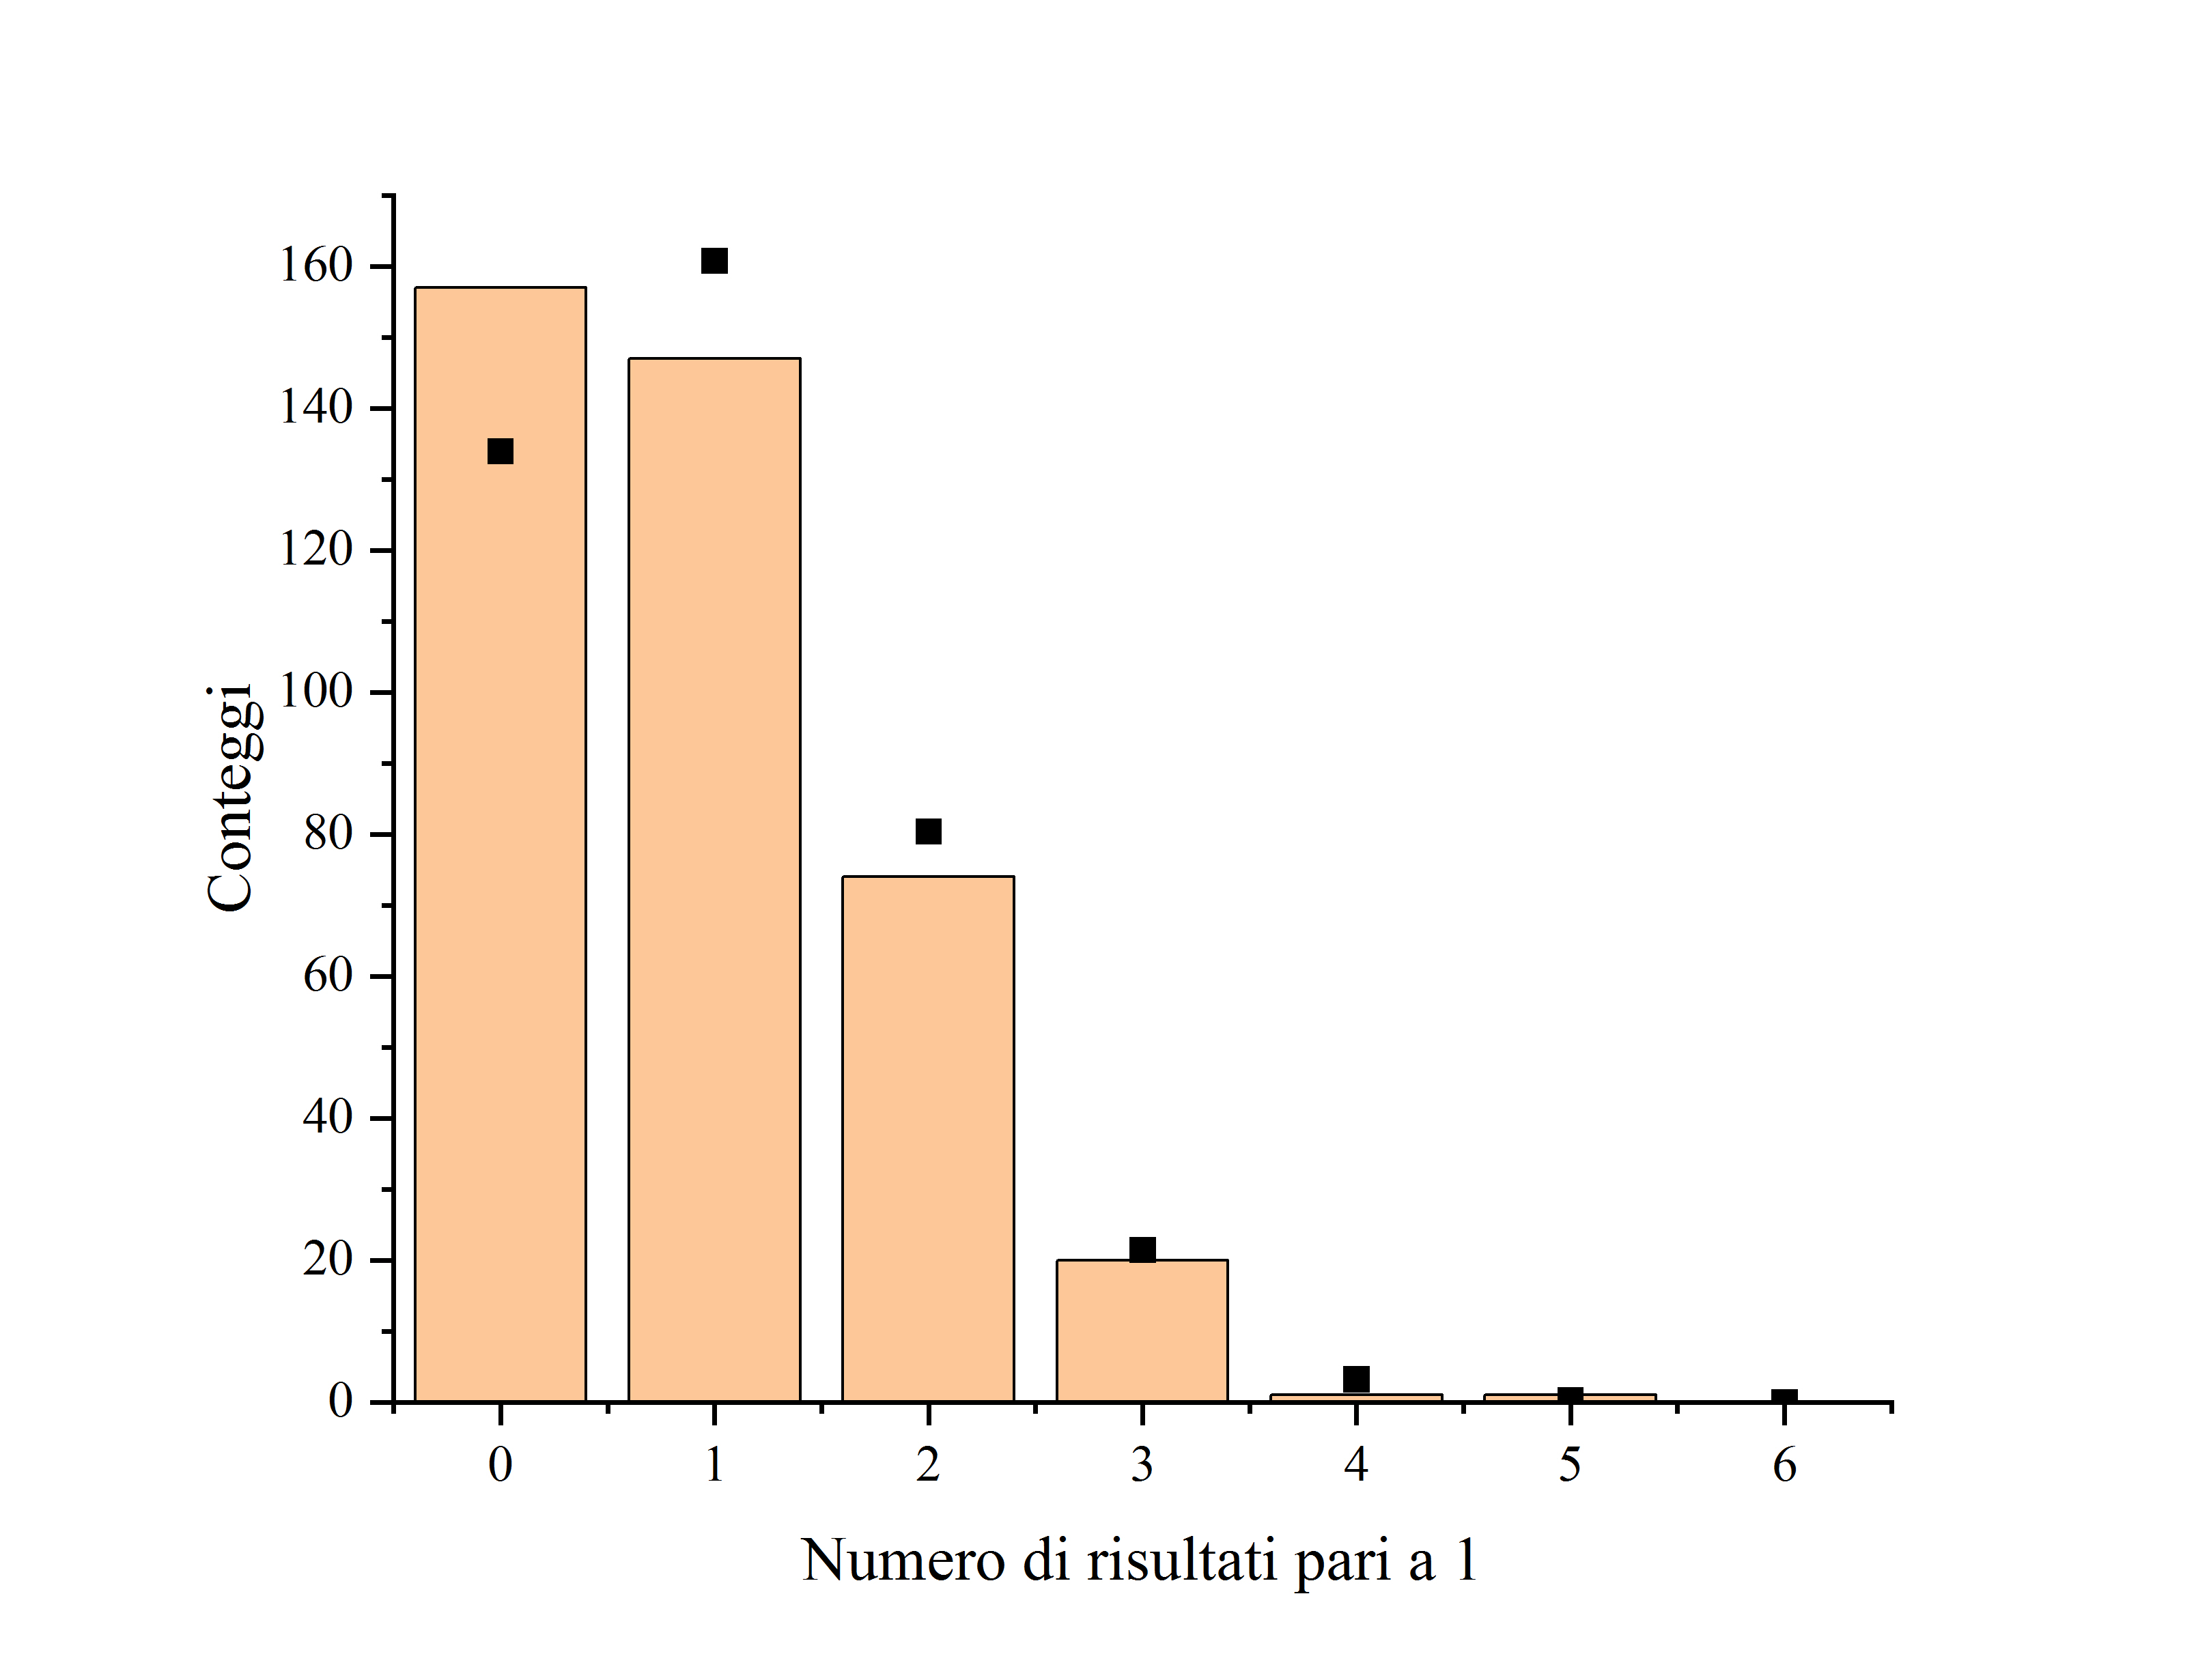
\includegraphics[trim={2cm .5cm 2.4cm 2.1cm},clip,width=.5\textwidth]{img/Dadi1.jpg}
        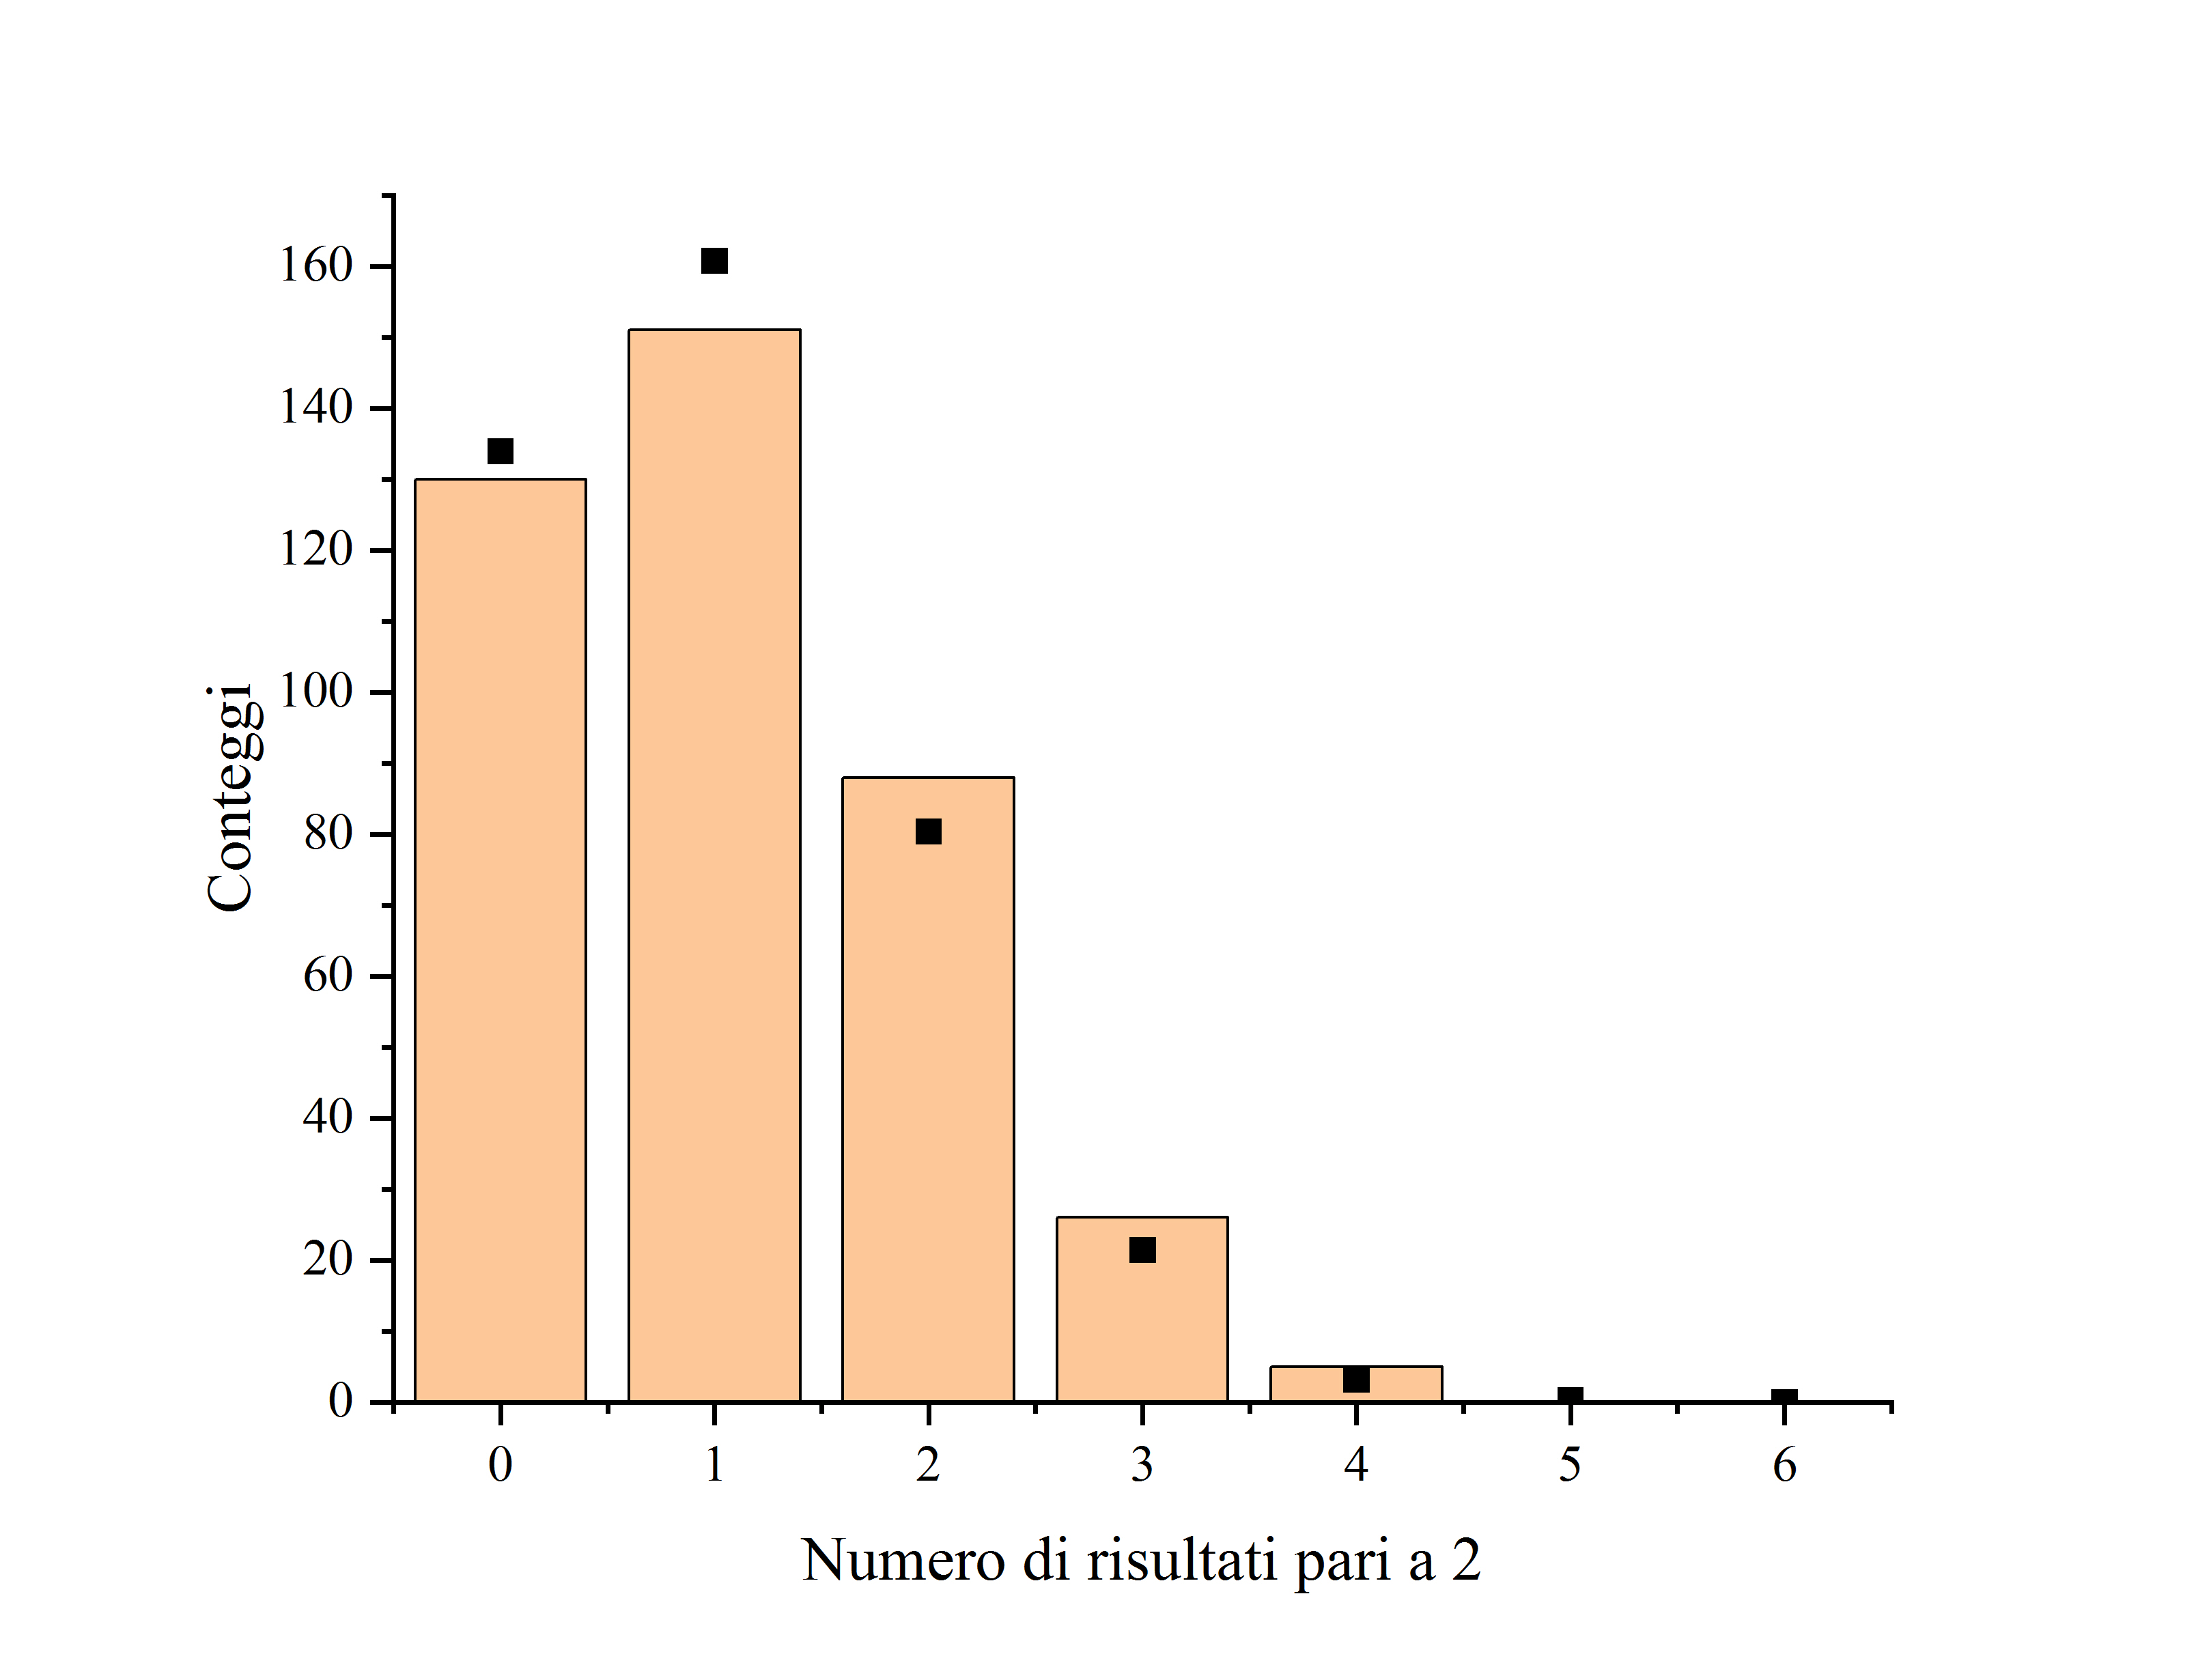
\includegraphics[trim={2cm .5cm 2.4cm 2.1cm},clip,width=.5\textwidth]{img/Dadi2.jpg}
        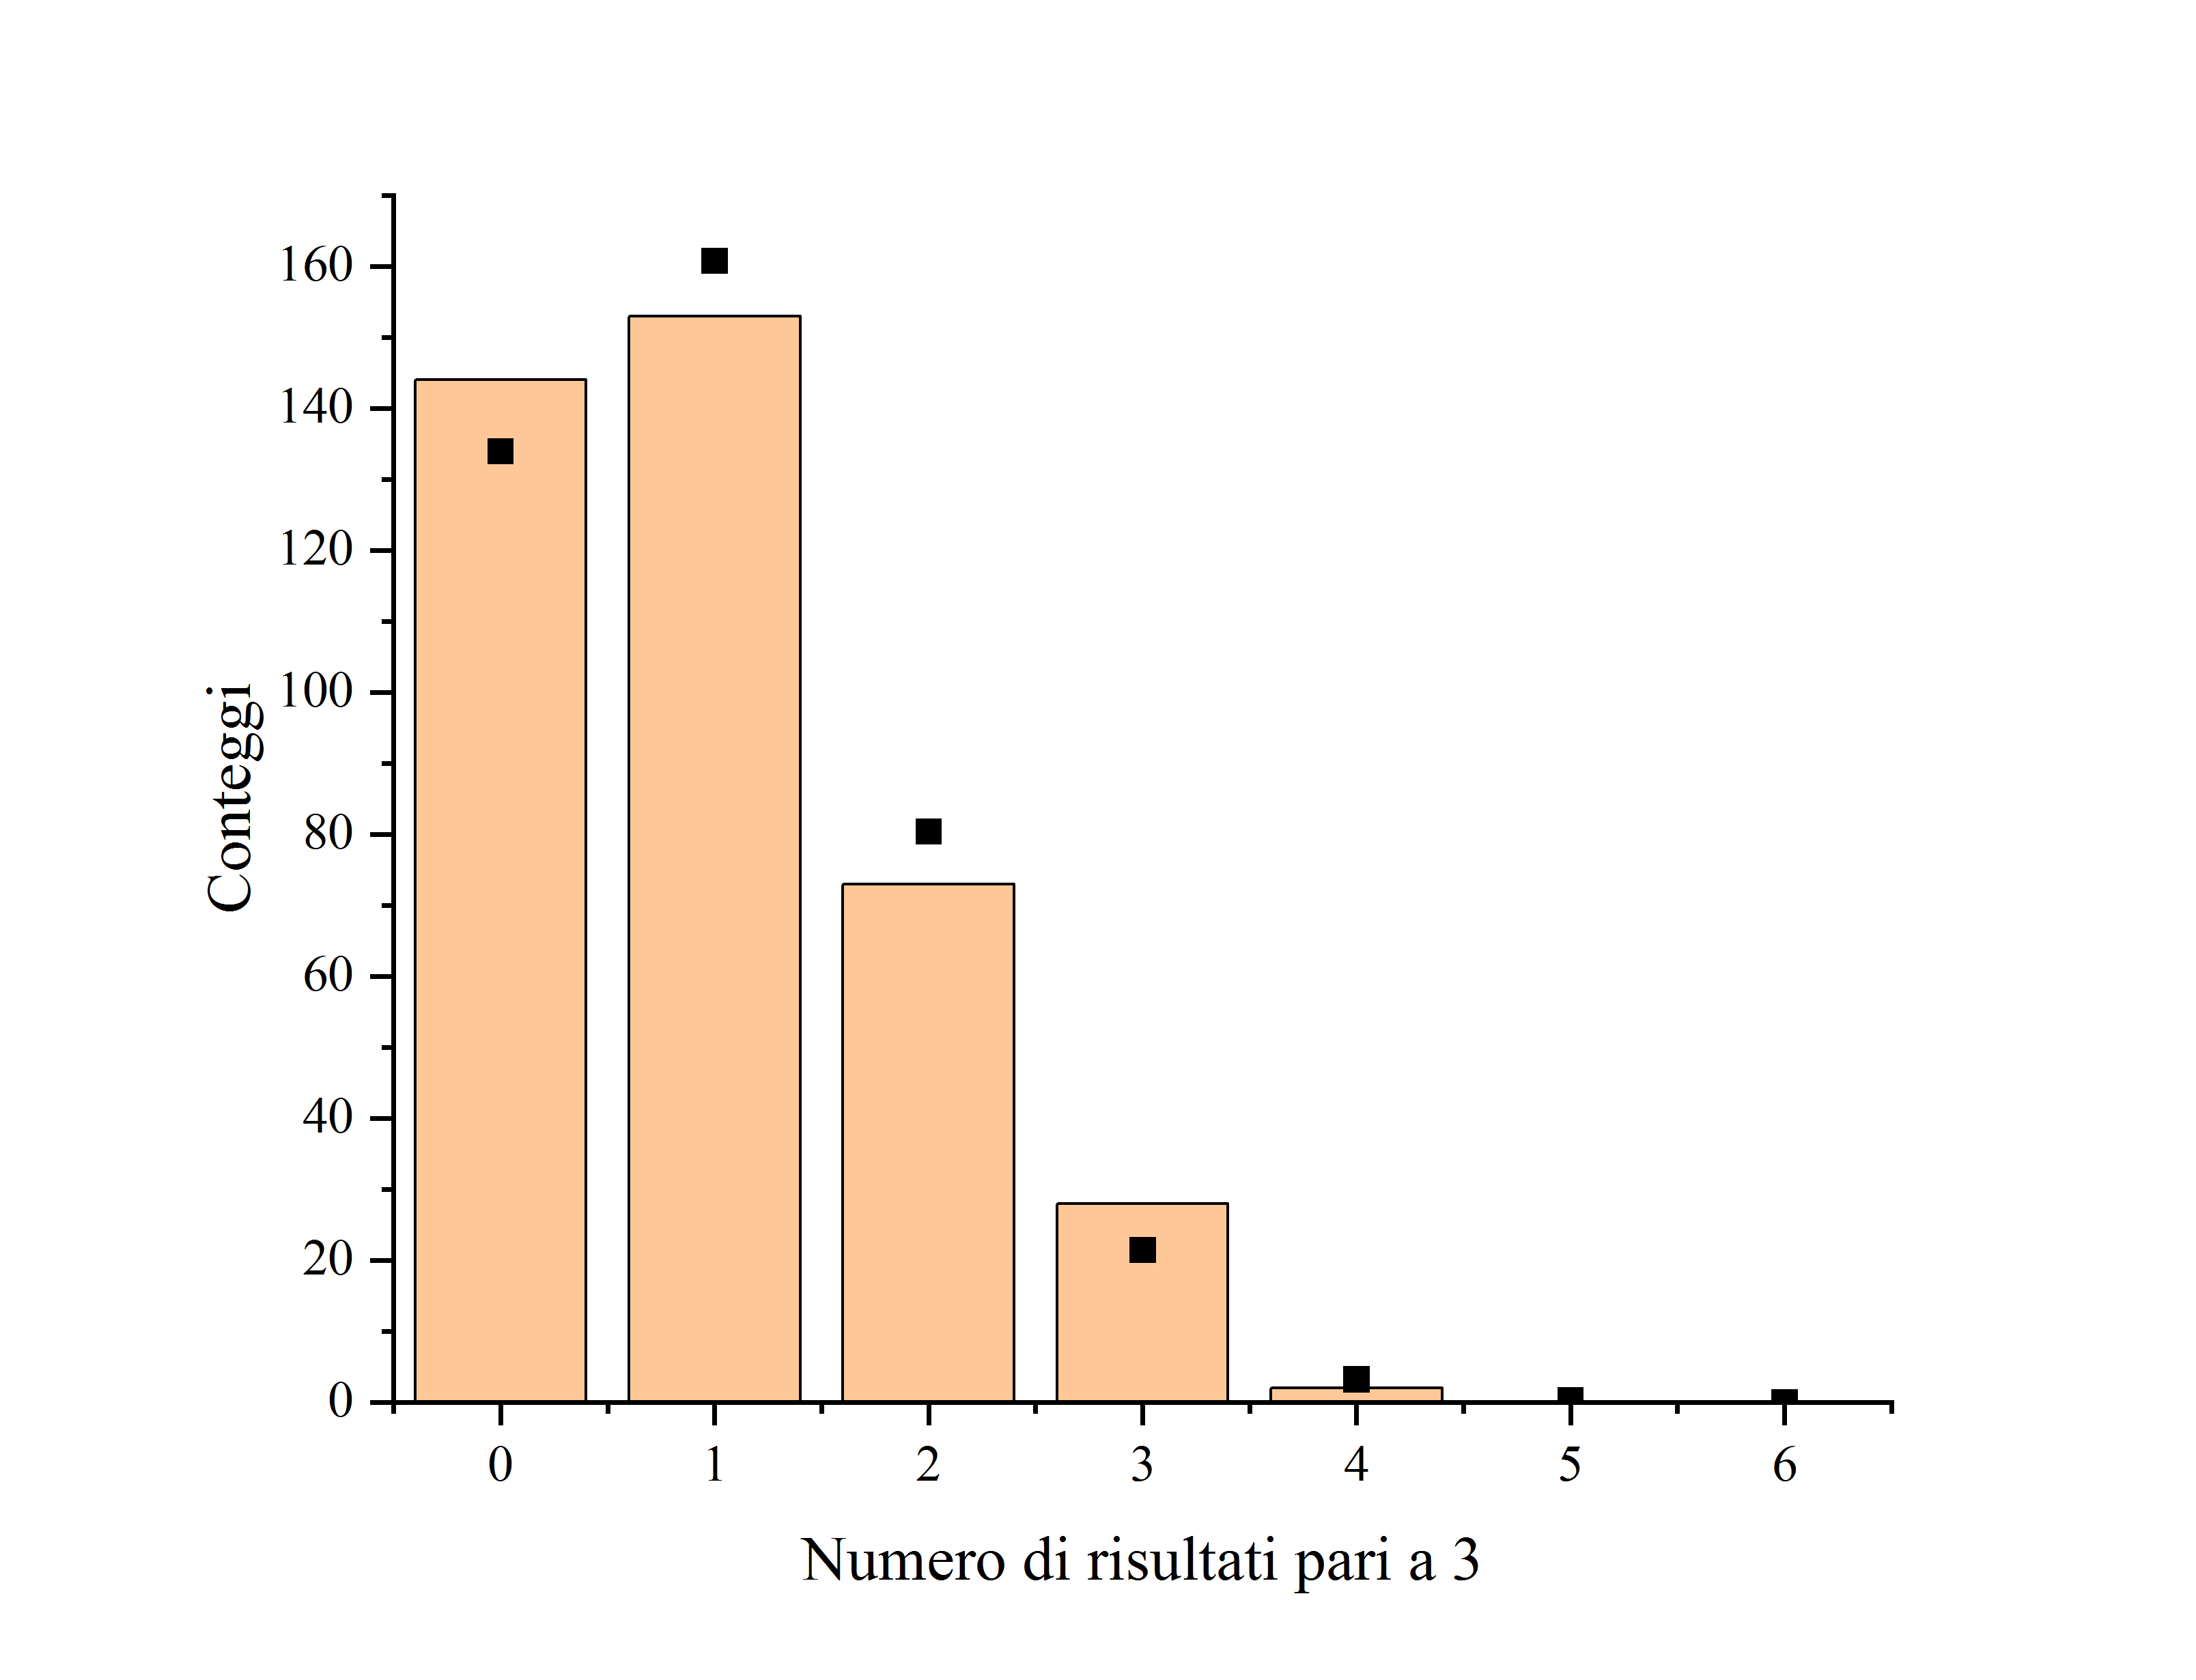
\includegraphics[trim={2cm .5cm 2.4cm 2.1cm},clip,width=.5\textwidth]{img/Dadi3.jpg}
        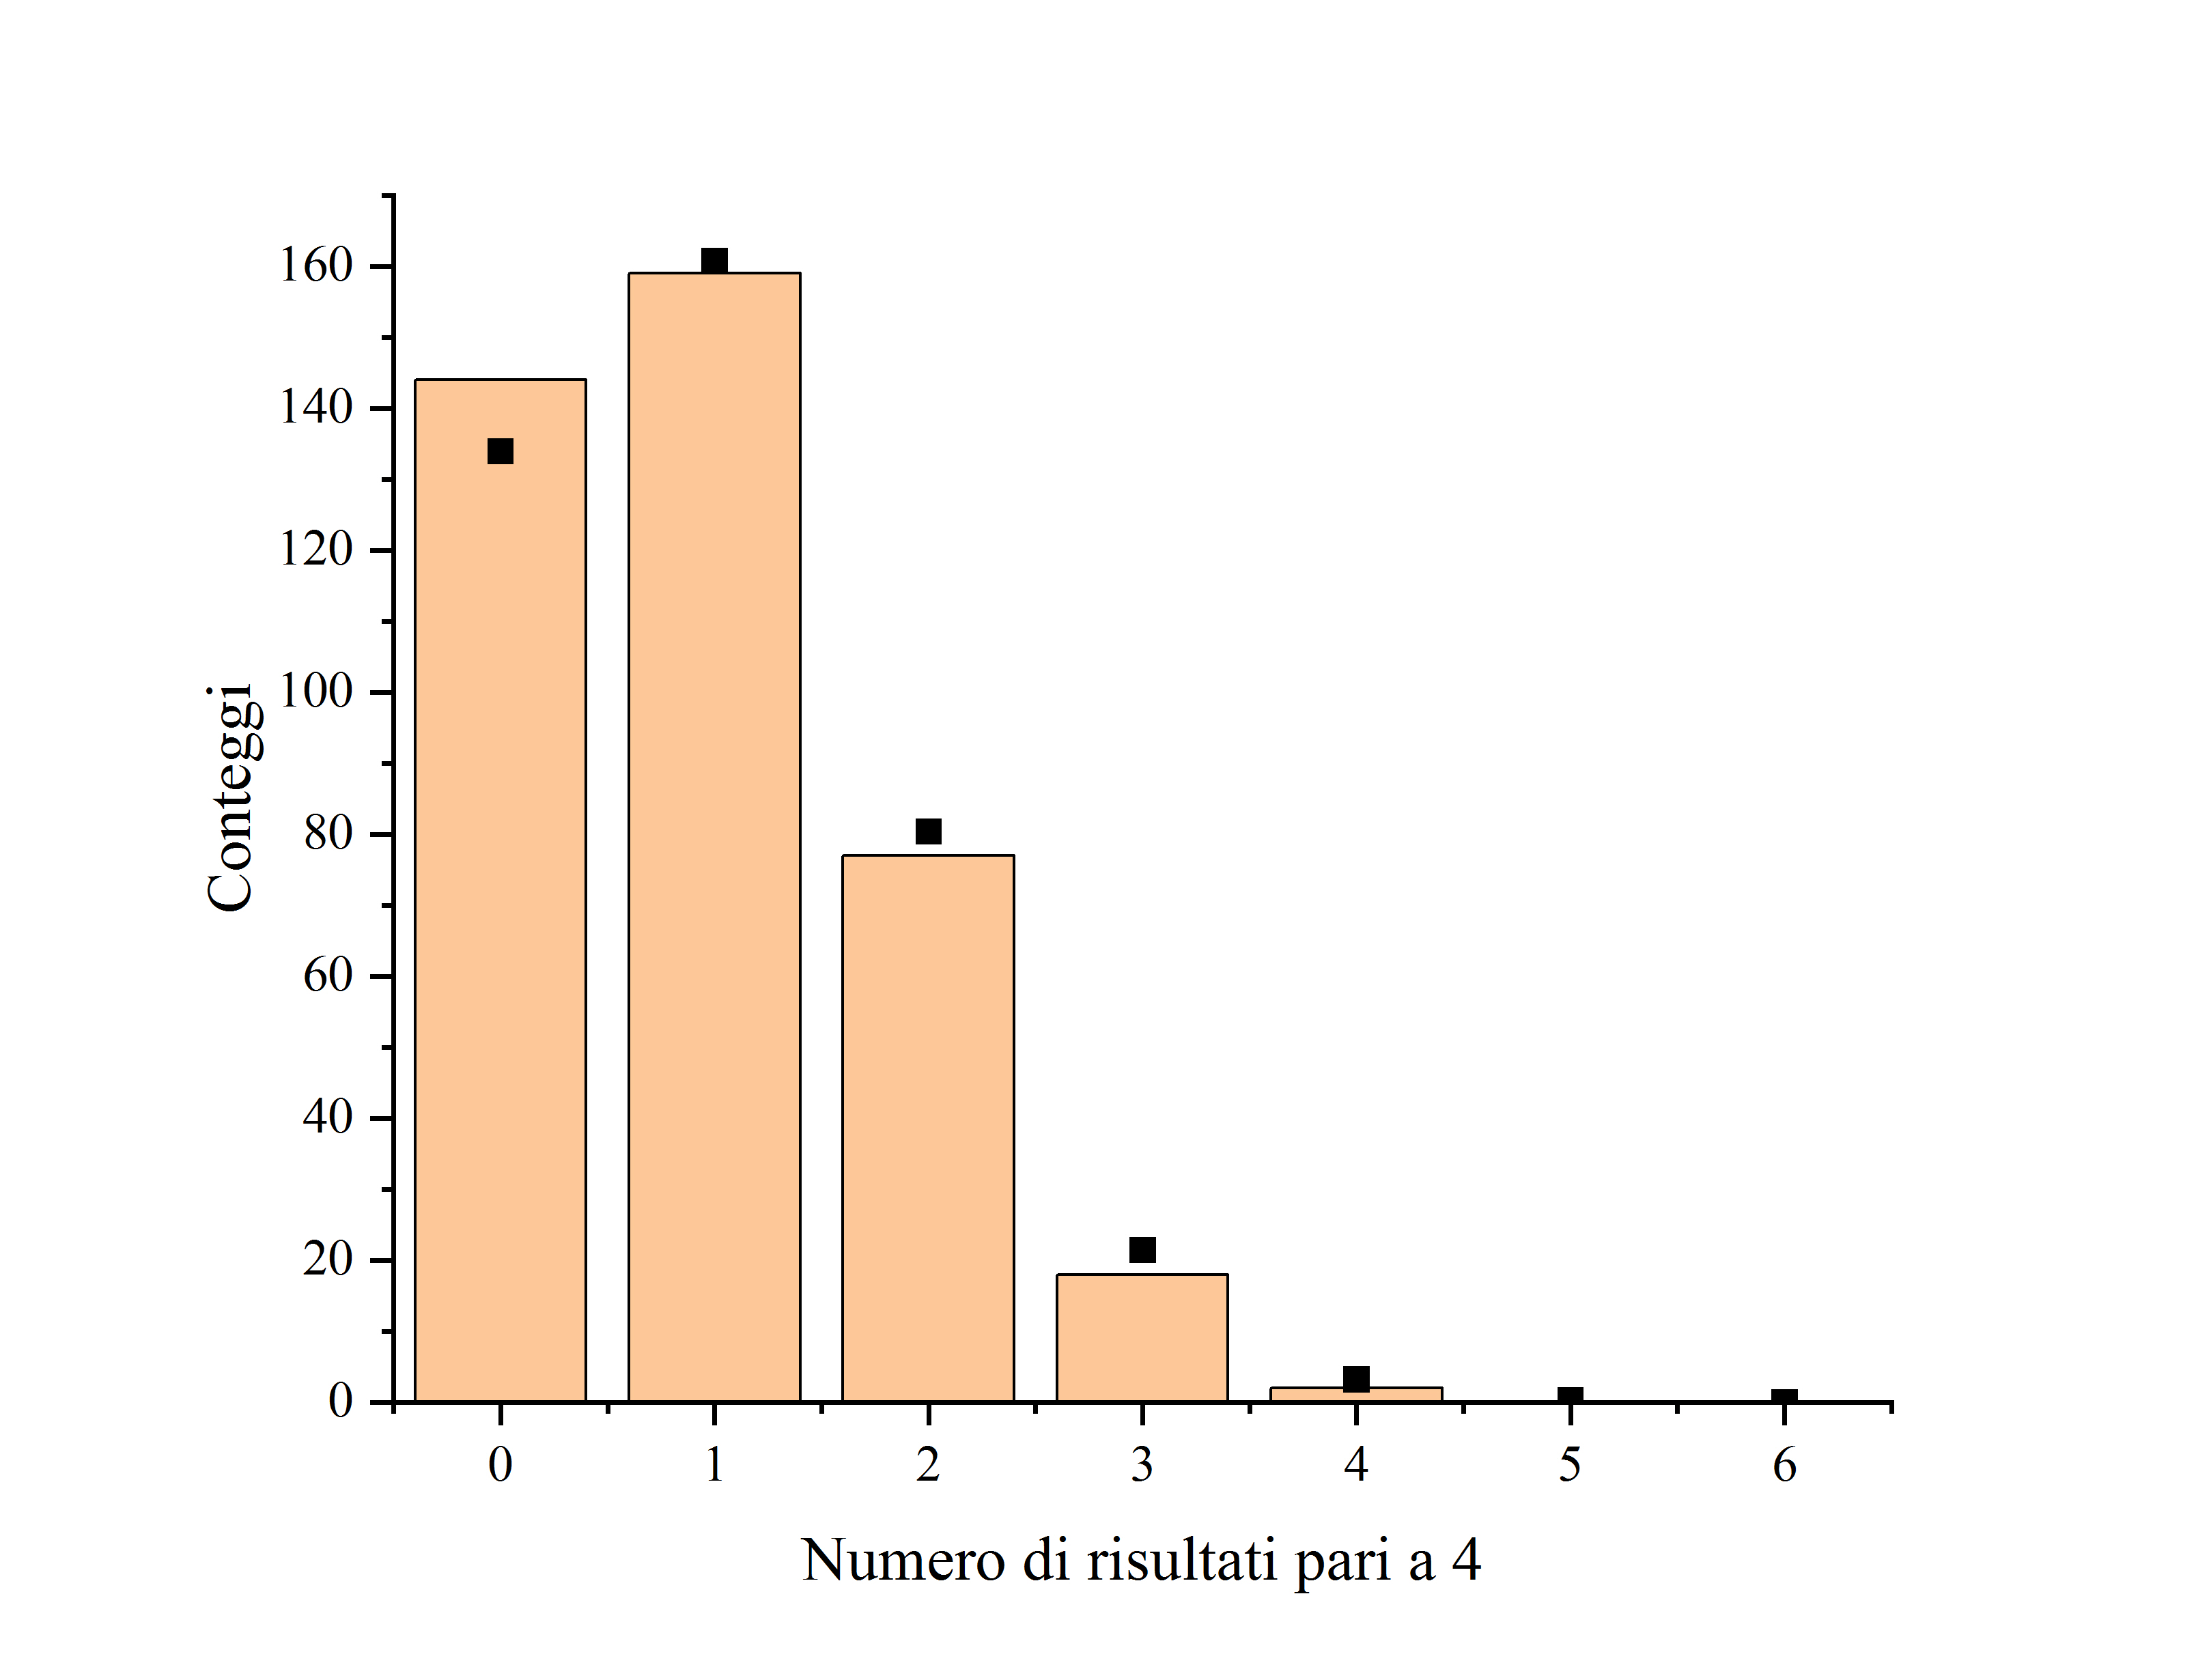
\includegraphics[trim={2cm .5cm 2.4cm 2.1cm},clip,width=.5\textwidth]{img/Dadi4.jpg}
        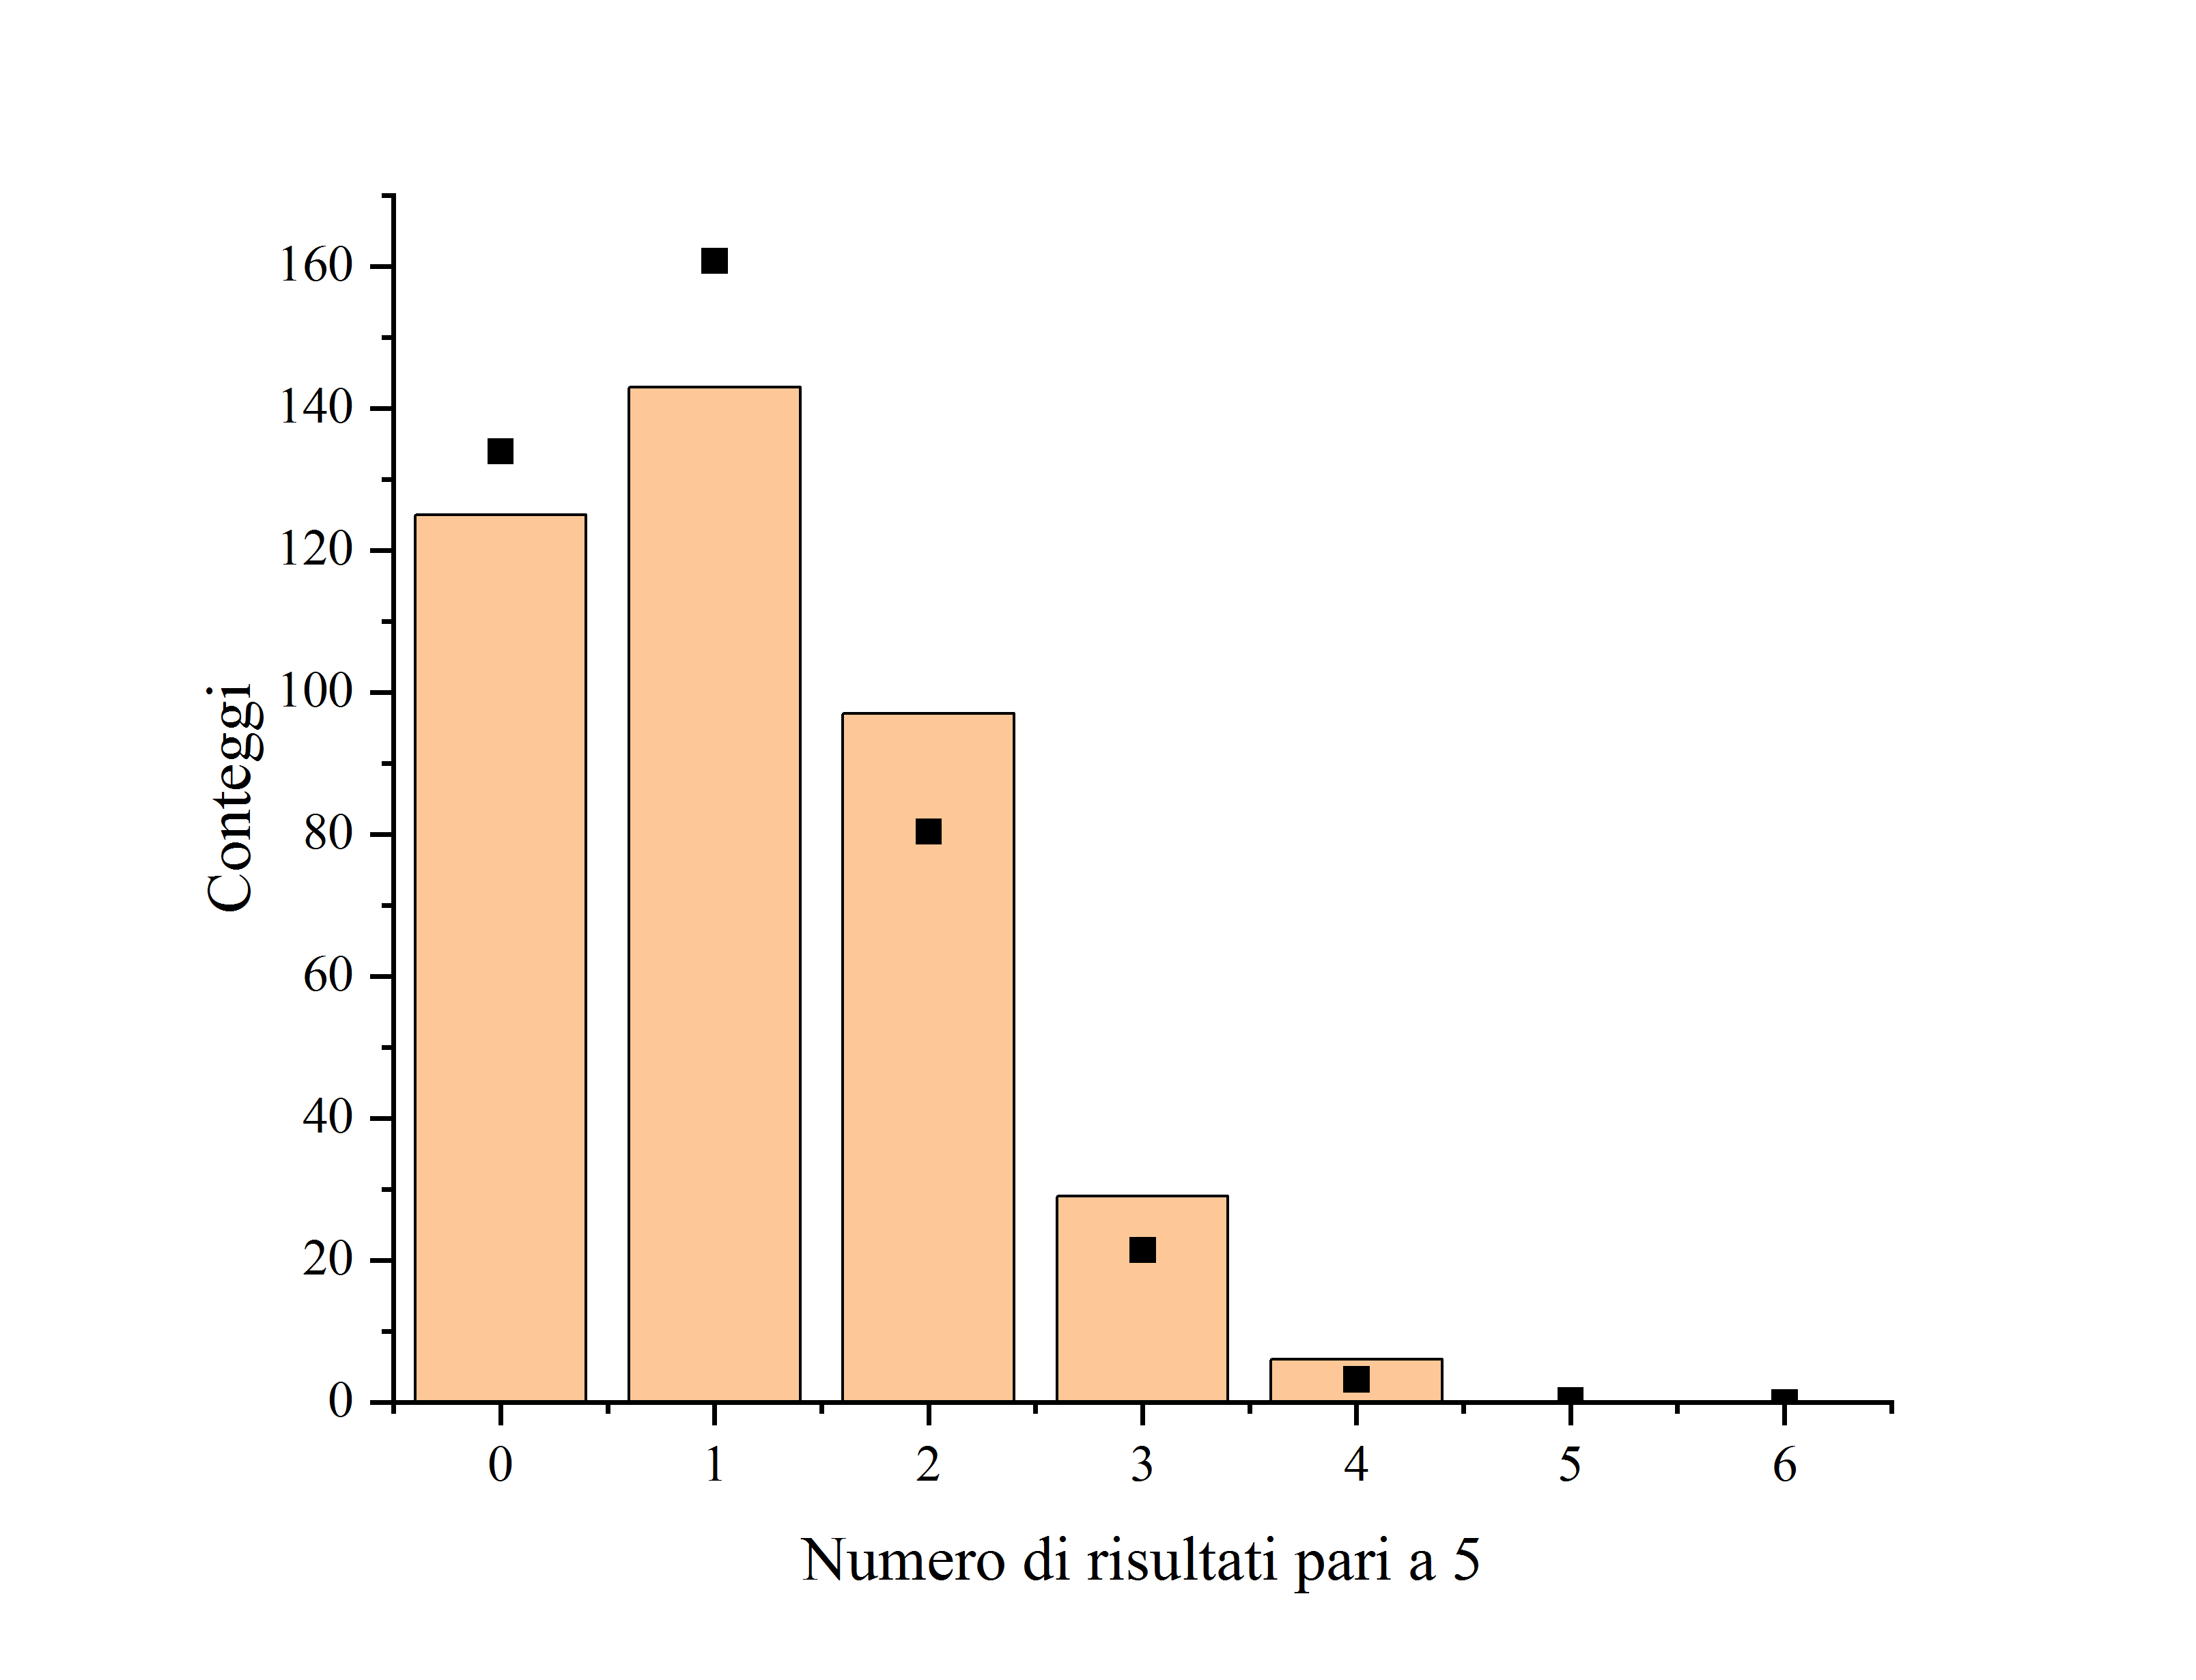
\includegraphics[trim={2cm .5cm 2.4cm 2.1cm},clip,width=.5\textwidth]{img/Dadi5.jpg}
        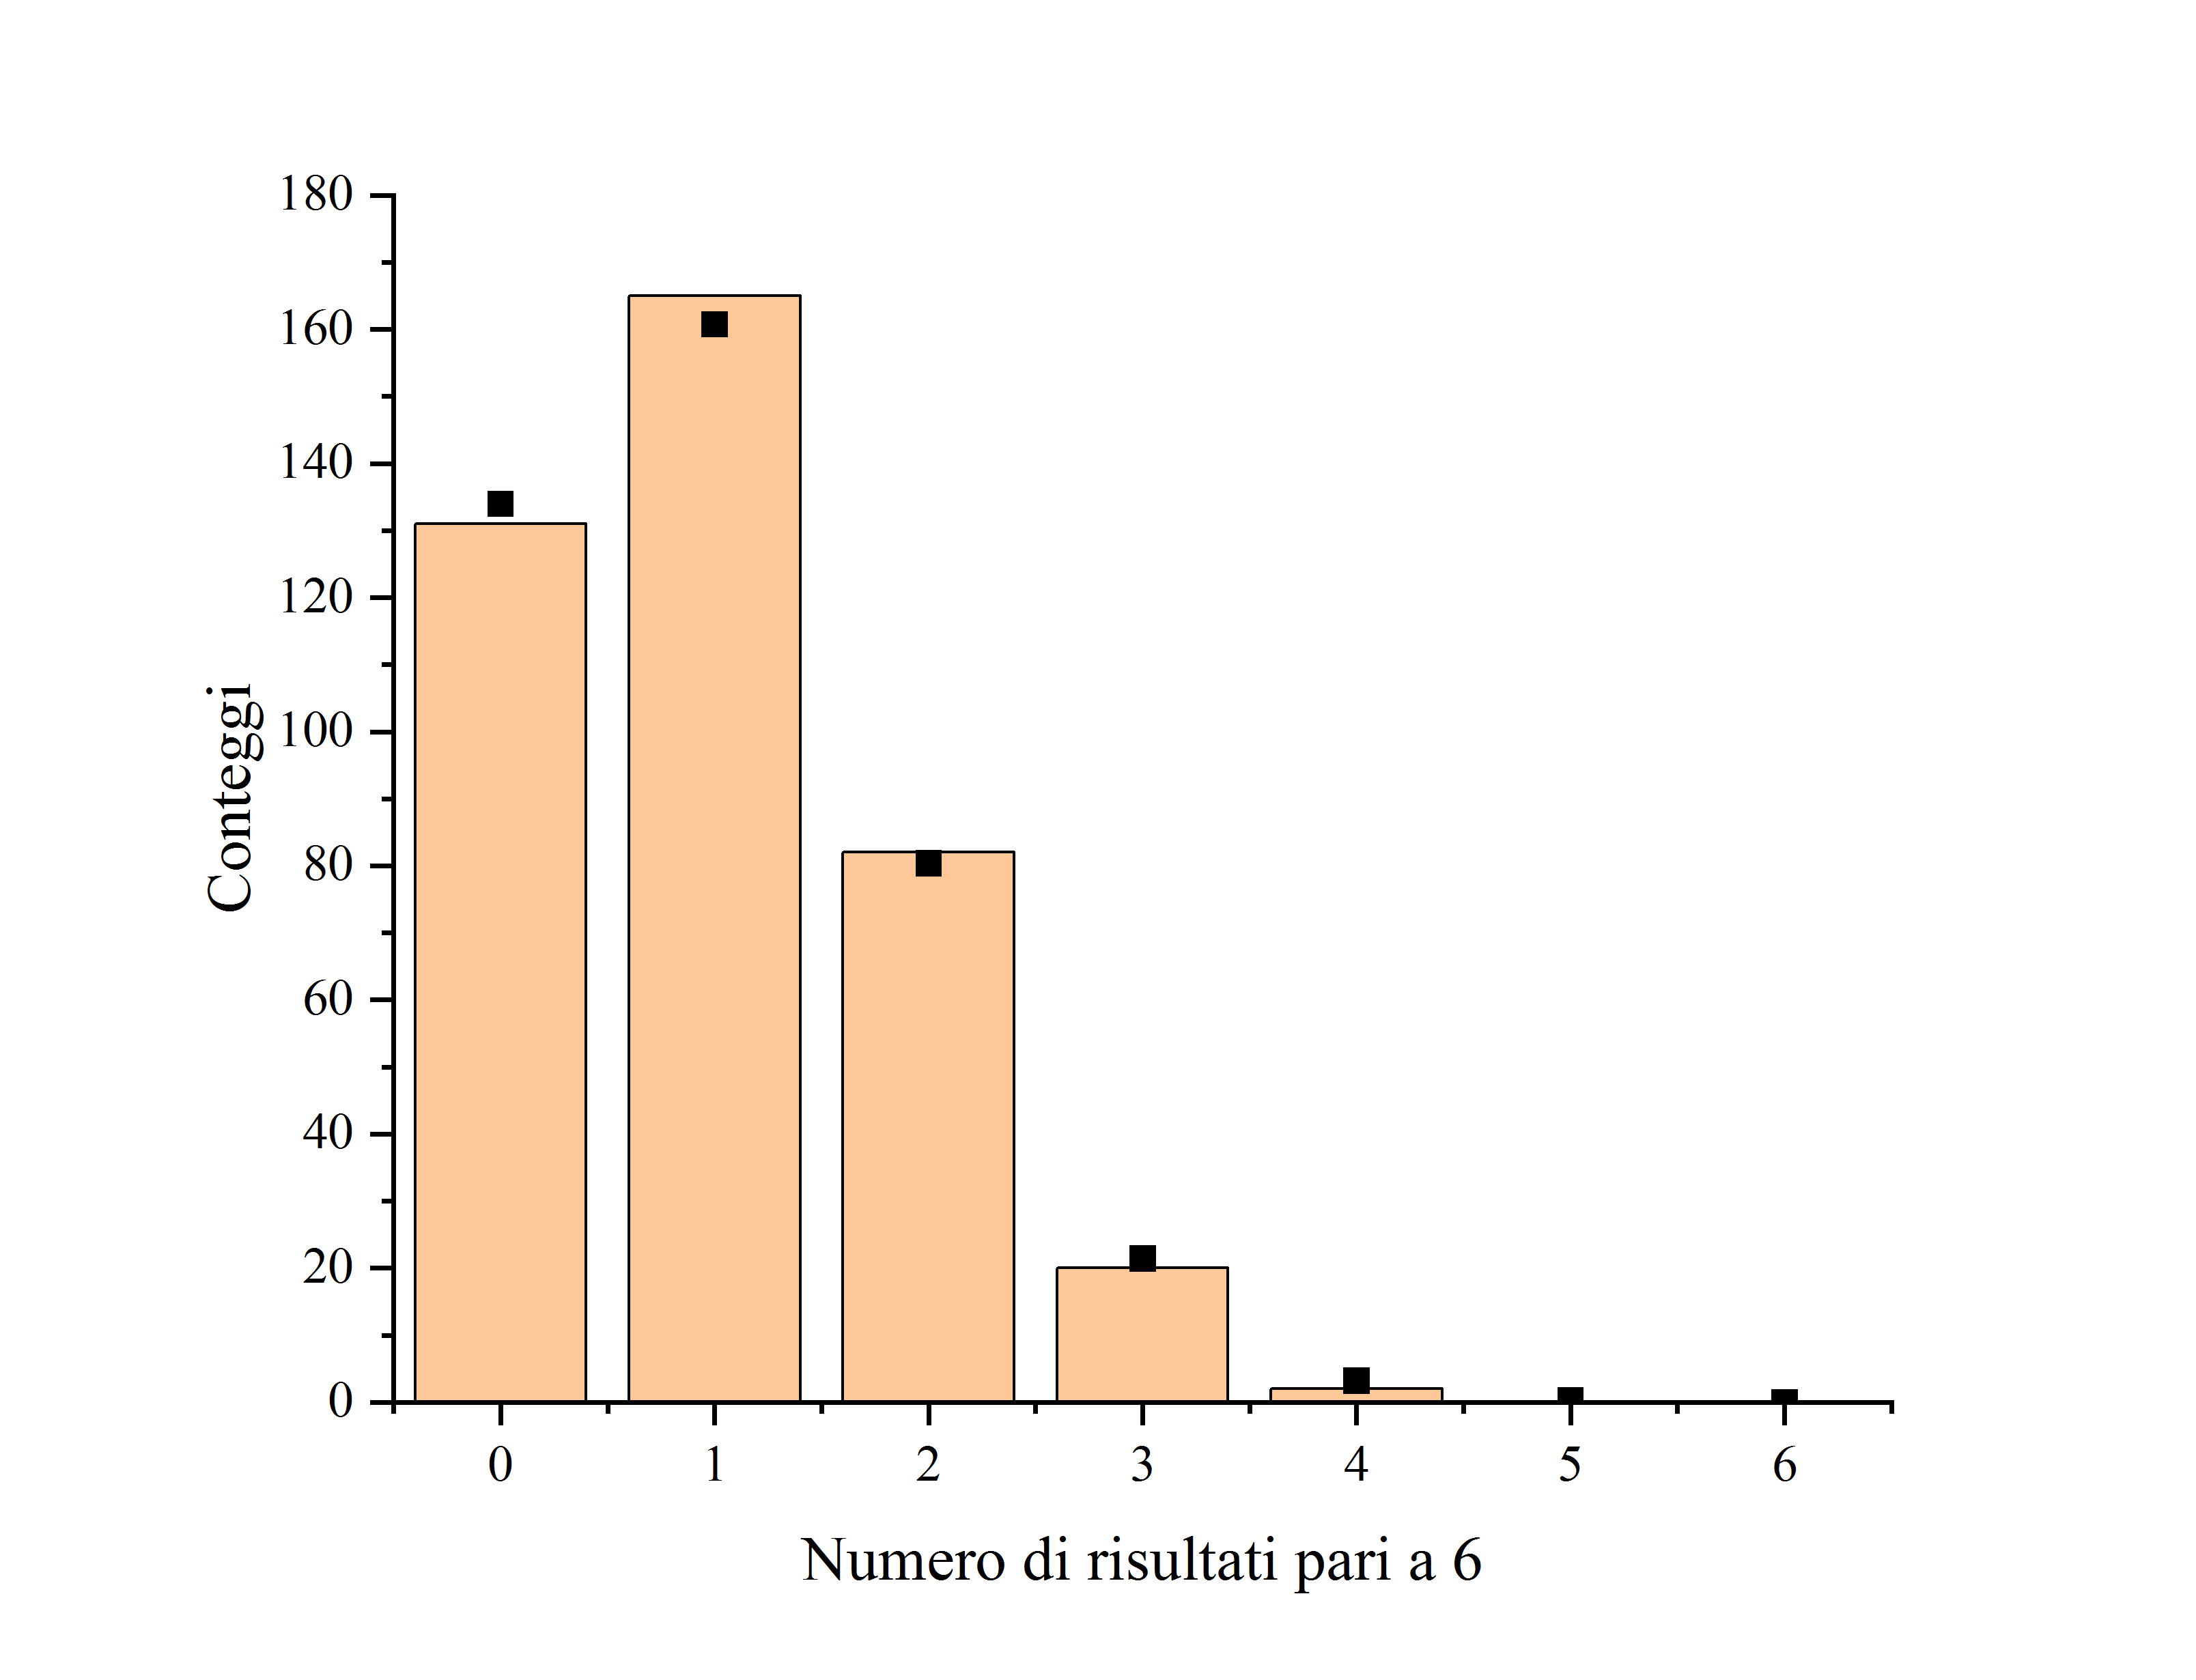
\includegraphics[trim={2cm .5cm 2.4cm 2.1cm},clip,width=.5\textwidth]{img/Dadi6.jpg}
    \end{figure}
\end{center}

Come è possibile osservare da questi grafici, i risultati riportati sembrano seguire
grossomodo la distribuzione teorica. Tuttavia, presentano deviazioni osservabili; il
gruppo di lavoro ritiene che ciò sia principalmente dovuto al ridotto numero di lanci.

\subsubsection*{Onestà dei dadi}
Avendo raccolto tutti i risultati di ogni dado, possiamo infine stimare se i dadi che
abbiamo utilizzato sono truccati o meno. Essendo questa analisi statistica solo
tangenziale rispetto al resto del lavoro, la riportiamo in dettaglio nell'appendice A.

\subsection{Simulazione}
Tramite un programma da noi scritto e compilato\footnote{\emph{Vedi} Appendice B},
simuliamo la stessa esperienza con $10^{12}$ lanci dei sei dadi, al fine di
verificare la legge dei grandi numeri.

Di seguito riportiamo, in un istogramma, i risultati della simulazione.

\begin{center}
    \begin{figure}[H]
        % trim={< v > ^}
        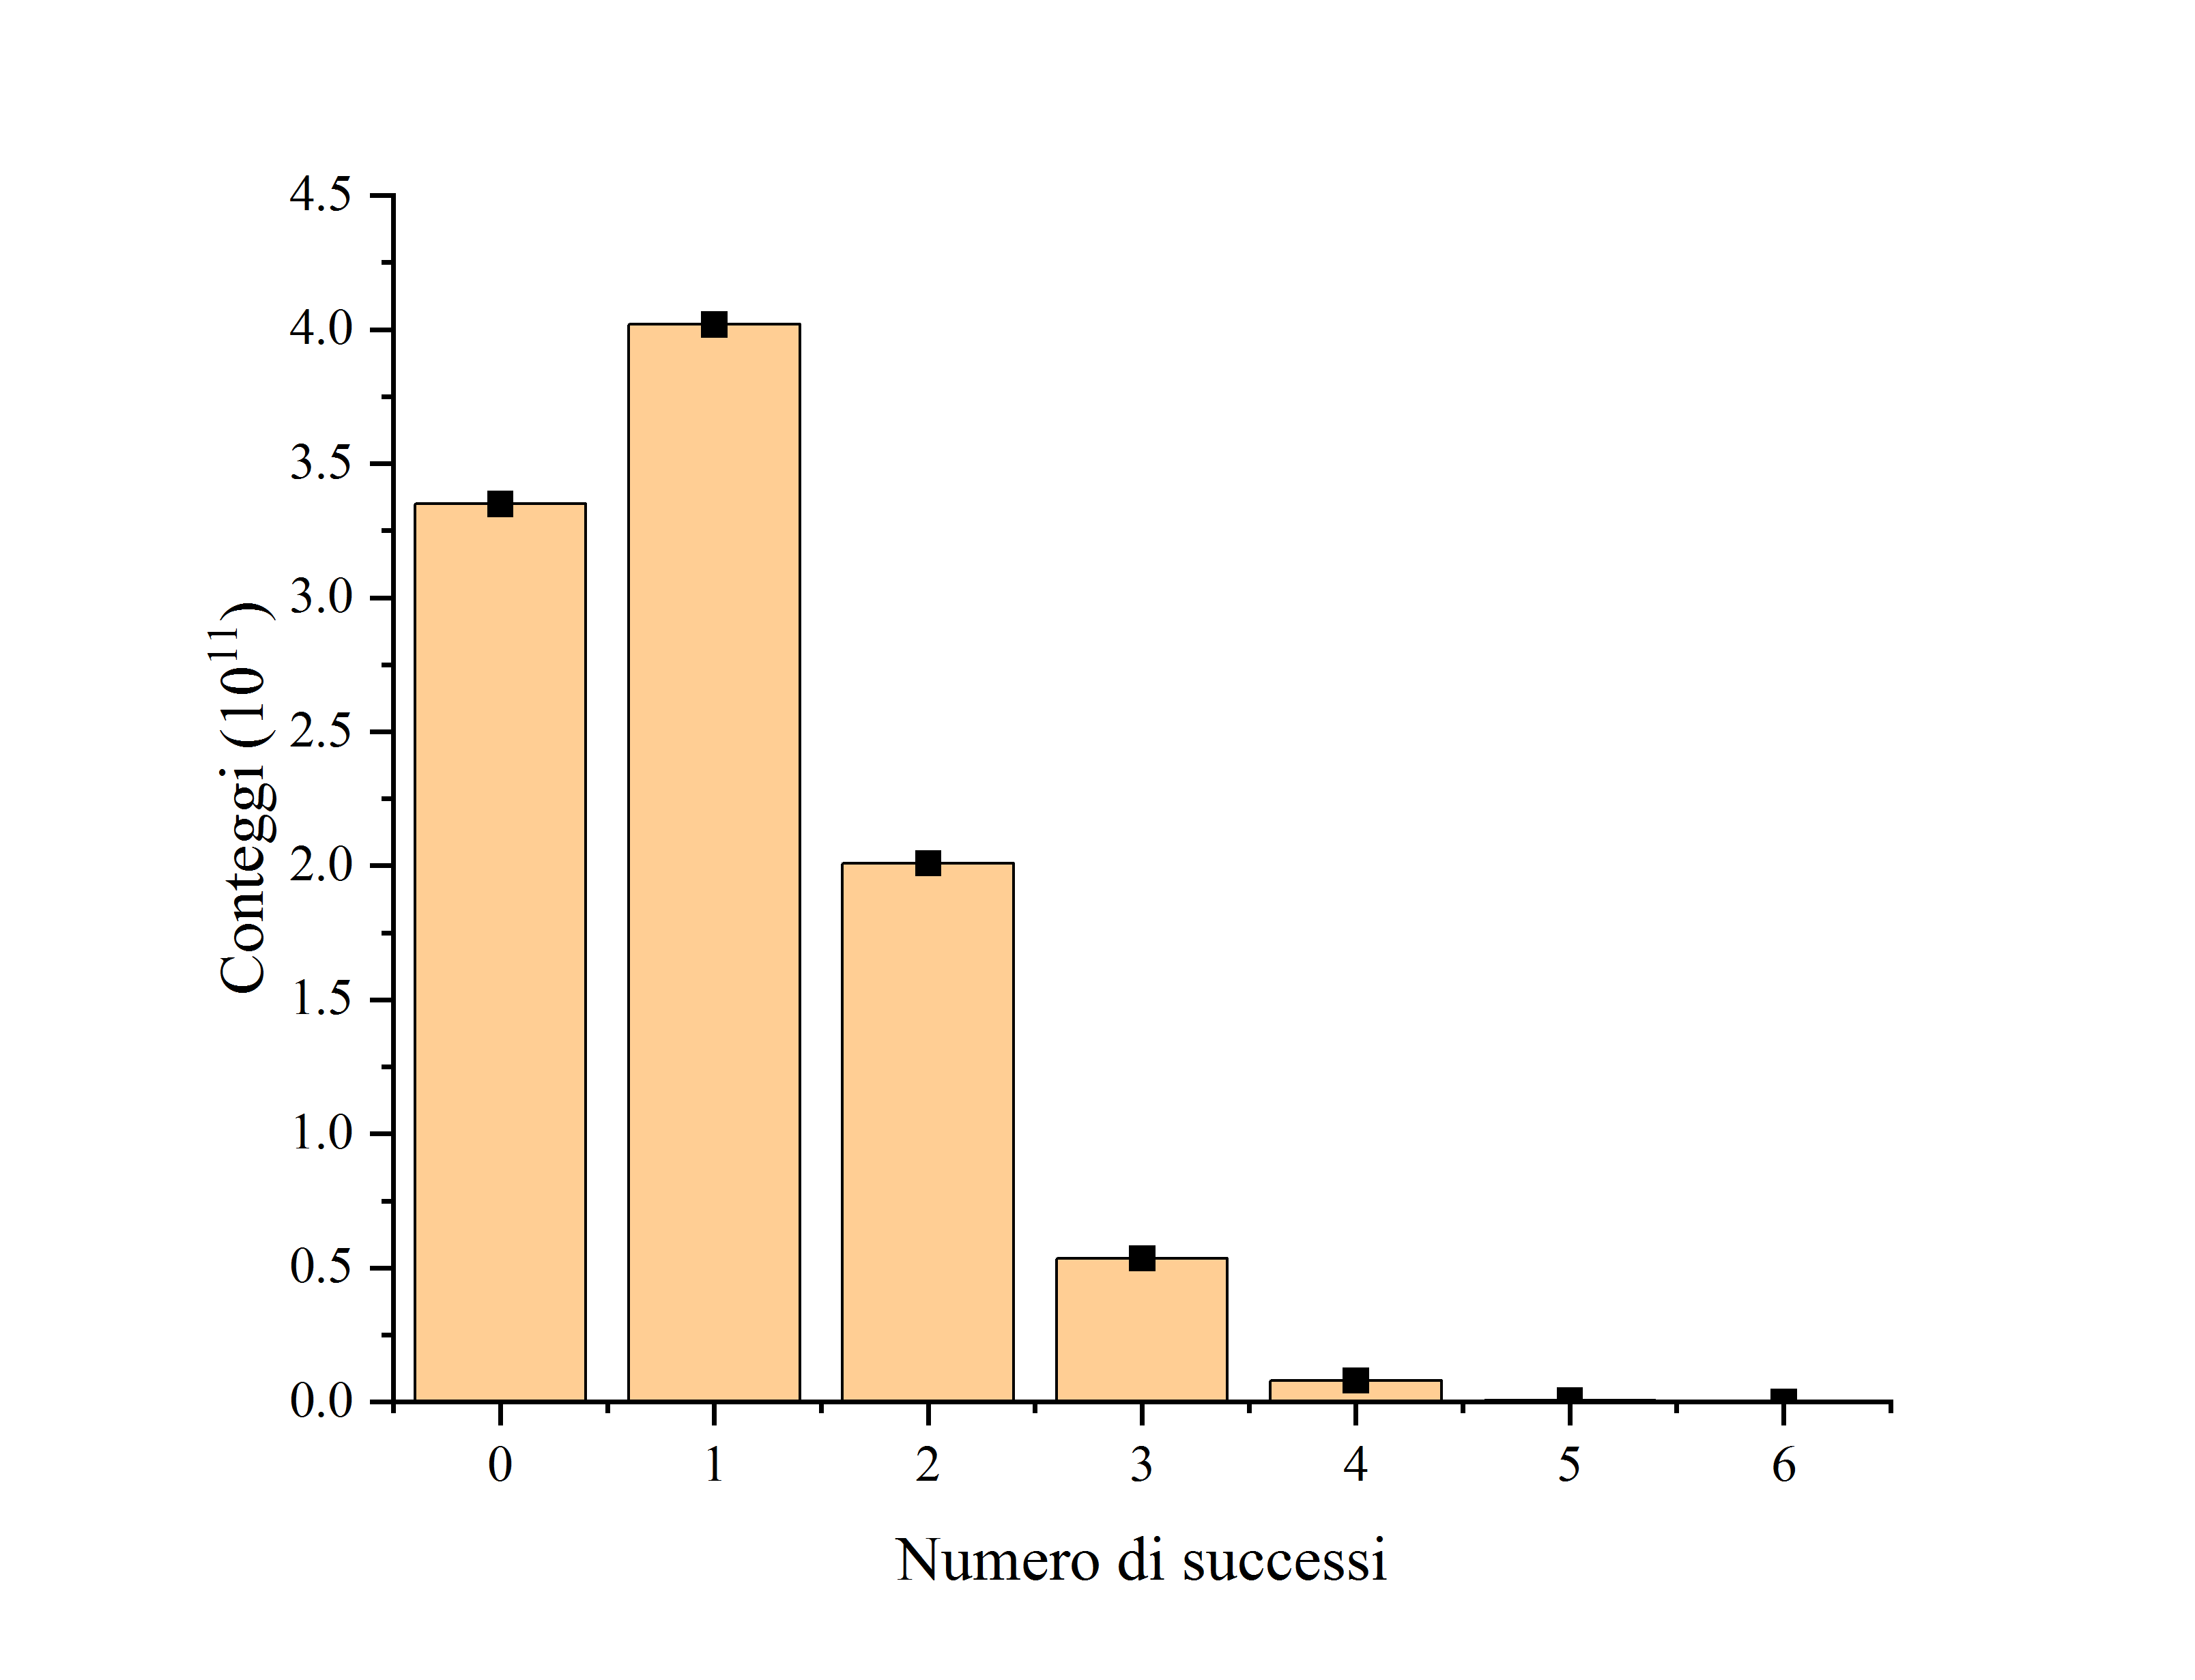
\includegraphics[trim={2cm .5cm 2cm 2.1cm},clip,width=\textwidth]{img/DadiSimul.png}
    \end{figure}
\end{center}

Come è possibile osservare dal grafico, i risultati della simulazione sono, in proporzione,
talmente vicini alla distribuzione teorica da risultare pressoché indistinguibili da essa.

Ciò è in accordo con la legge dei grandi numeri, secondo la quale, al crescere del
numero di prove, la distribuzione di probabilità rappresenta sempre meglio i
risultati ottenuti, normalizzati.

\pagebreak
\section{Processo di Poisson}
\subsection{Materiali e strumenti di misura utilizzati}
\begin{center}
    \begin{tblr}{ |Q[l,m]|Q[c,m]|Q[c,m]|Q[c,m]| }
        \hline
        \textbf{Strumento di misura} & \textbf{\:\:\:\:\:Soglia\:\:\:\:\:} & \textbf{Portata} & \textbf{Sensibilità} \\
        \hline
        {Contatore Geiger} & \qty{1}{conteggi \per s} & N./A. & \qty{1}{conteggi \per s} \\
        \hline[dashed]
        Metro a nastro & \qty{0.1}{cm} & \qty{300.0}{cm} & \qty{0.1}{cm} \\
        \hline
        \hline
        \textbf{Altro} & \SetCell[c=3]{l} \textbf{Descrizione/Note} \\
        \hline
        {Campione di $\Th$} & \SetCell[c=3]{l} {
            Componente di una lampada da campeggio
        } \\
        \hline
    \end{tblr}
\end{center}


\subsection{Esperienza e procedimento di misura}

Posizionato il contatore Geiger a una certa distanza $d_i$ dal campione di $\Th$
(con $i\in\left[1;4\right]\cap\mathbb{N}$),
definiamo una variabile aleatoria\footnote{
    L'unità di misura di $x_i$ (e, conseguentemente, anche di $\overline{x_i}$) è
    $\unit{s^{-1}}$. Detto altrimenti,
    $x_i\in\left\{n\,\unit{s^{-1}}:n\in\mathbb{N}\right\}$
} $x_i$ come il numero di raggi $\gamma$
emessi dal $\Th$ nell'arco di un secondo, nella direzione del contatore.
Allora, detta $\overline{x_i}$ la media teorica
% \footnote{
    % Che il parametro della distribuzione coincida con la media è facilmente
    % dimostrabile. Detto $\lambda$ quel parametro, vale:
    % \[\begin{aligned}
        % \overline{x_\gamma} &= \sum_{k=0}^{+\infty} k\,p(x_\gamma=k) =
        % \sum_{k=0}^{+\infty} k \frac{\lambda^k  e^{-\lambda}}{k!} =
        % e^{-\lambda} \sum_{k=0}^{+\infty} k \frac{\lambda^k}{k!} =
        % e^{-\lambda} \left(0 + \sum_{k=1}^{+\infty} k \frac{\lambda^k}{k!}\right) \\ &=
        % \lambda e^{-\lambda} \sum_{k=1}^{+\infty} \frac{\lambda^{k-1}}{(k-1)!} =
        % \lambda e^{-\lambda} \sum_{j=0}^{+\infty} \frac{\lambda^j}{j!} =
        % \lambda e^{-\lambda} e^\lambda =
        % \lambda\quad\square
    % \end{aligned}\]
% }
di $x_i$, la distribuzione di probabilità di $x_i$ è data da una Poissoniana:
\[
    p(x_i=k)=\frac{\overline{x_i}^k e^{-\overline{x_i}}}{k!}
    \qquad
    \forall k\in\mathbb{N}
\]
Il valore di $\overline{x_i}$ è legato alla distanza $d_i$, al raggio $r$
della finestra del contatore, al tempo di dimezzamento $T_\frac{1}{2}$ del
$\Th$ e al numero $N$ di atomi di $\Th$ secondo la seguente relazione\footnote{
    Il numero medio $\overline{X}$ di raggi $\gamma$ emessi dal campione è
    $\overline{X} = \tau^{-1}N = {T^{-1}_\frac{1}{2}}N\ln{2}$,
    con $\tau=\frac{1}{\ln{2}}T_\frac{1}{2}$ il tempo caratteristico del $\Th$.
    Tuttavia, poiché la superficie di acquisizione è $\pi r^2$, e non $4\pi d_i^2$,
    dobbiamo moltiplicare per il rapporto fra le aree:
    \[
        \overline{x_i} = \frac{\pi r^2}{4\pi d_i^2} \overline{X} =
        \frac{Nr^2\ln{2}}{4 d_i^2 T_\frac{1}{2}}
    \]
    Infine, dobbiamo ricordare che il contatore Geiger non rileva soltanto le
    radiazioni emesse dal campione. Possiamo tenere conto di tutti gli altri
    contributi introducendo un termine costante $\overline{x_0}$, che chiameremo
    “media dei conteggi relativi alla radioattività ambientale”.
    Si ottiene così la relazione riportata.
}:
\[
    \overline{x_i} = \frac{Nr^2\ln{2}}{4 d_i^2 T_\frac{1}{2}} + \overline{x_0}
\]
D'ora in avanti indicheremo con $\xi$ la costante $\frac{Nr^2\ln{2}}{4T_\frac{1}{2}}$
(unità di misura: $\unit{m^2\per s}$).
La relazione diventa allora:
\[\overline{x_i} = \xi d_i^{-2} + \overline{x_0}\]

Per ogni distanza $d_i$, il gruppo di lavoro ha acquisito ripetutamente il valore di
$x_i$ per un tempo complessivo di circa un'ora\footnote{
    Abbiamo scelto deliberatamente di acquisire esattamente 3657 secondi in quanto
    $3657$ minimizza la funzione
    $f(x)=\left\{\frac{x}{\pi}\right\}=\frac{x}{\pi} - \left\lfloor\frac{x}{\pi}\right\rfloor$
    meglio di $3600$.
} ($\qty{3657}{s}$); ha poi acquisito nuovamente $x_4$ col contatore Geiger rivolto in
direzione opposta, per avere una stima diretta di $\overline{x_0}$.

Di seguito riportiamo gli istogrammi dei dati così raccolti,
assieme ai valori attesi, calcolati mediante la distribuzione teorica.

\begin{center}
    \begin{figure}[H]
        % trim={< v > ^}
        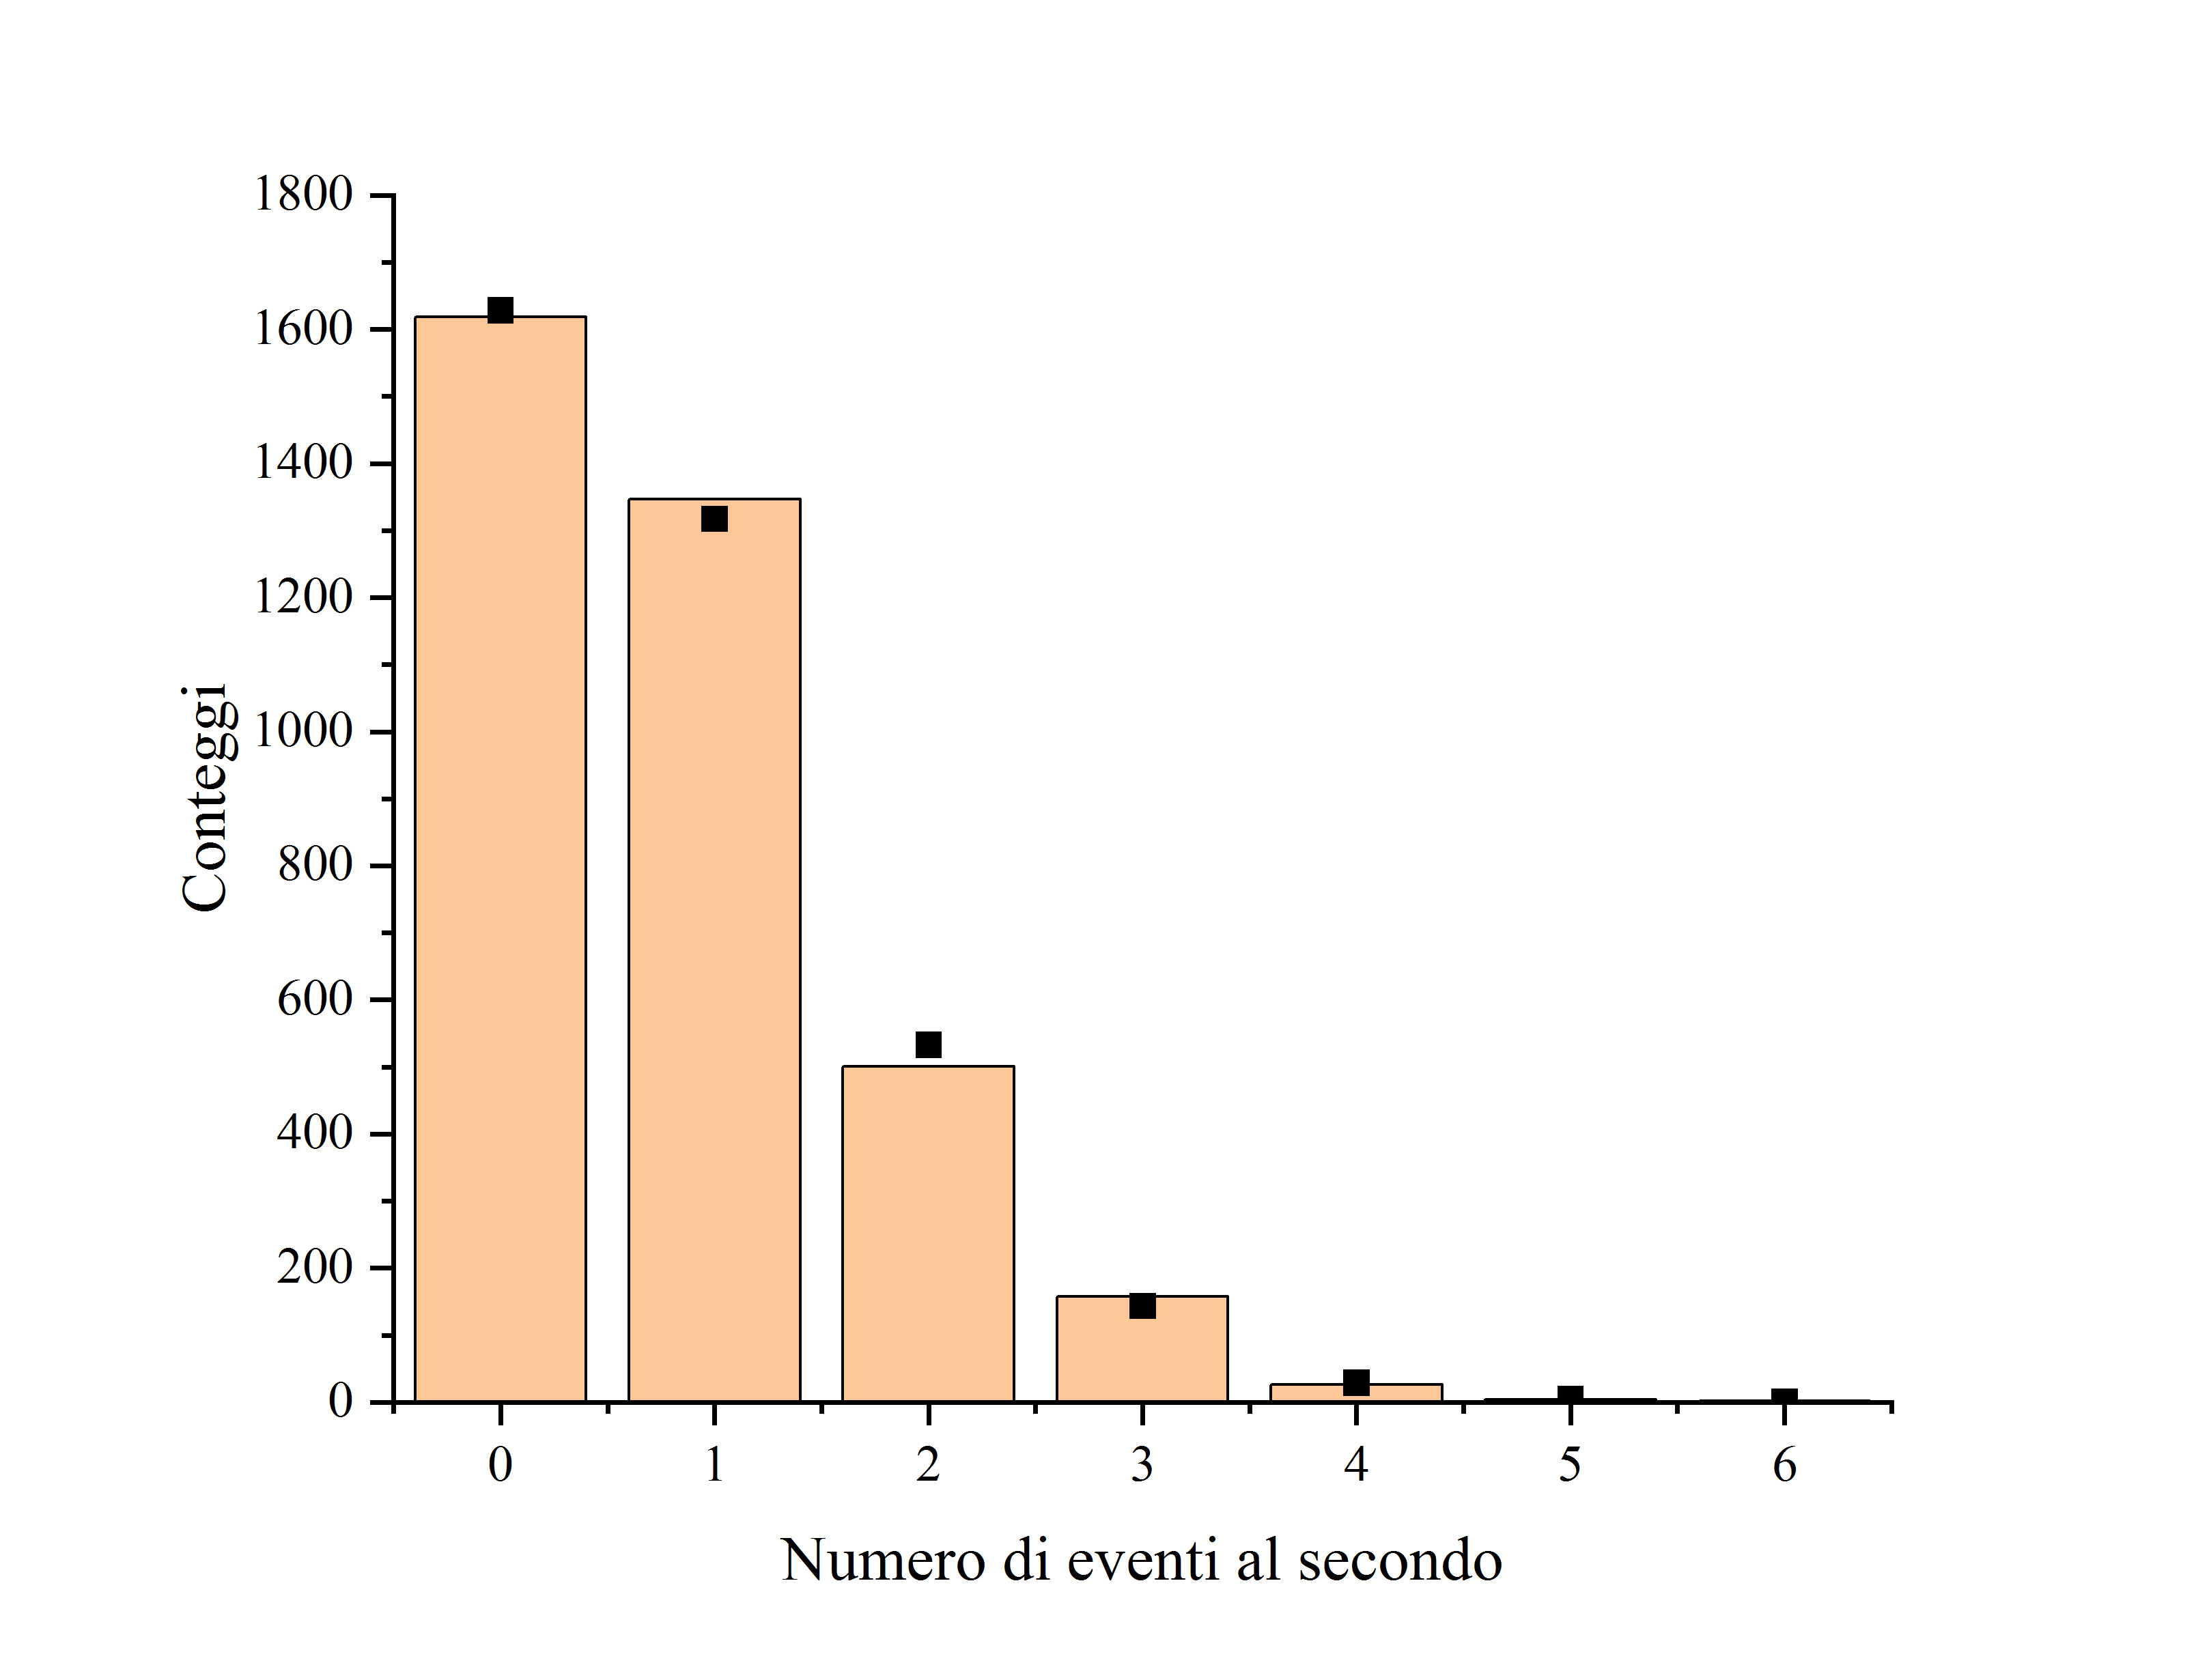
\includegraphics[trim={2cm .5cm 2.4cm 2.1cm},clip,width=.5\textwidth]{img/Geiger2.jpg}
        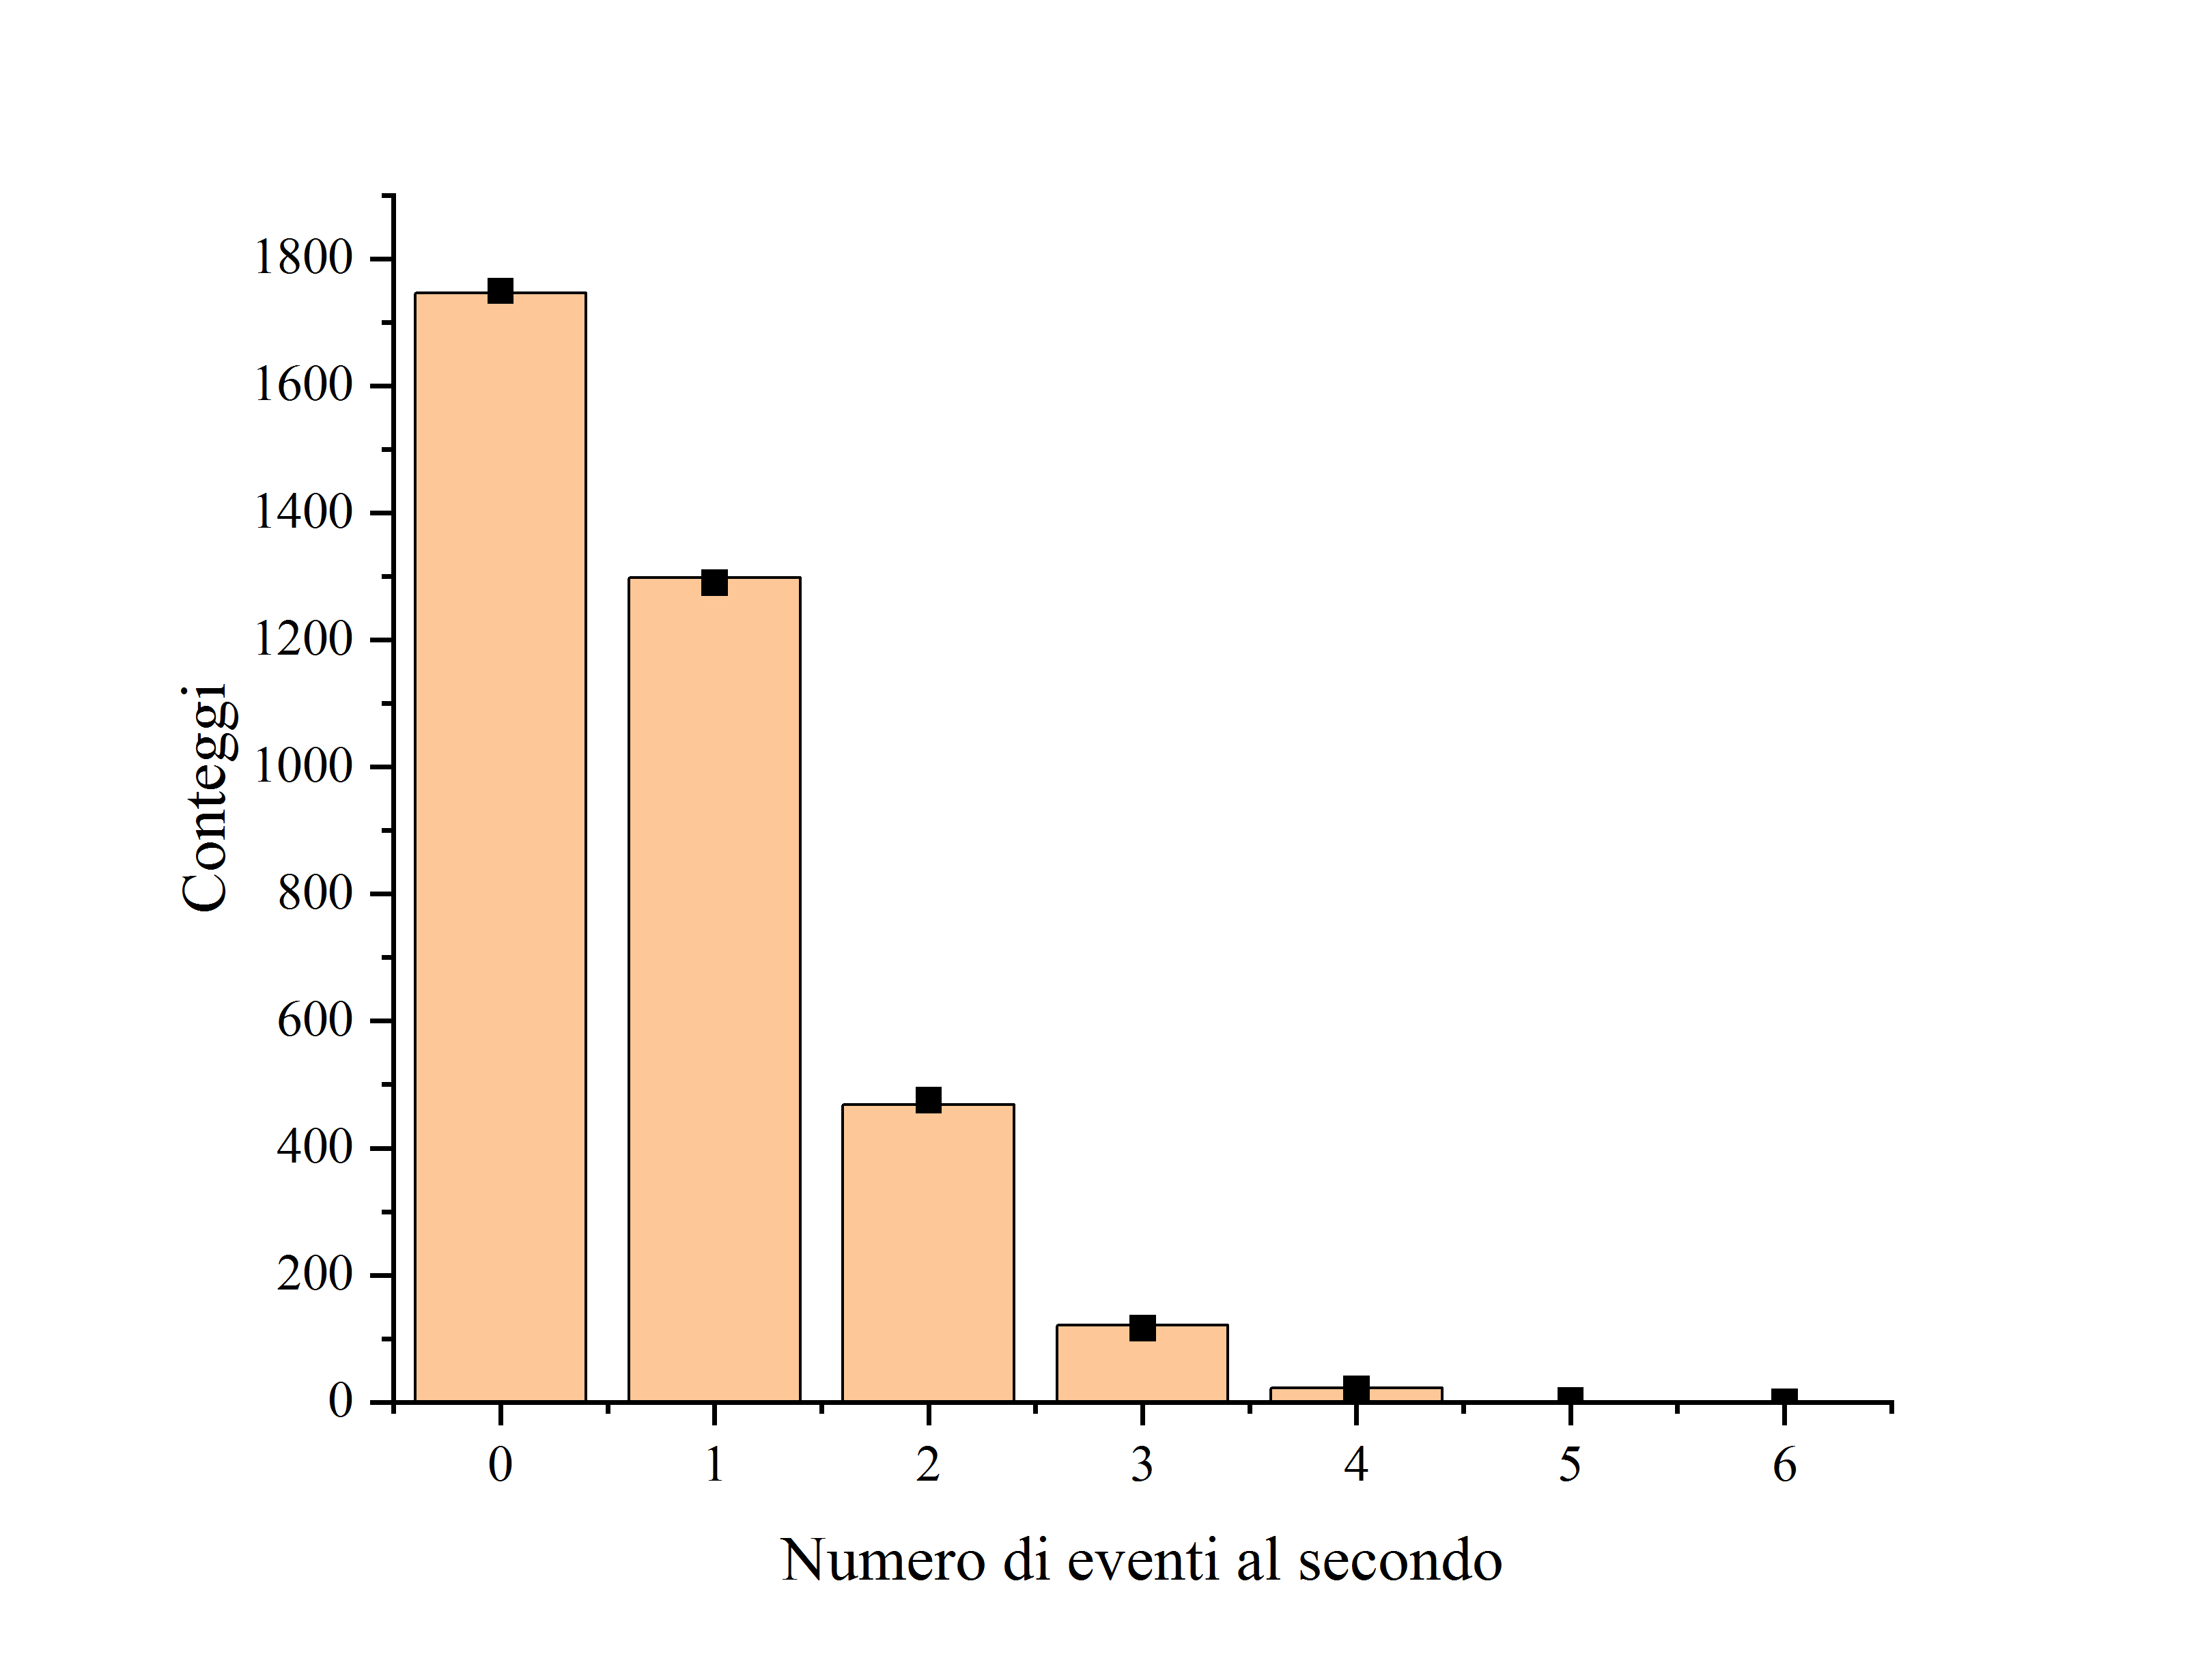
\includegraphics[trim={2cm .5cm 2.4cm 2.1cm},clip,width=.5\textwidth]{img/Geiger1.jpg}
        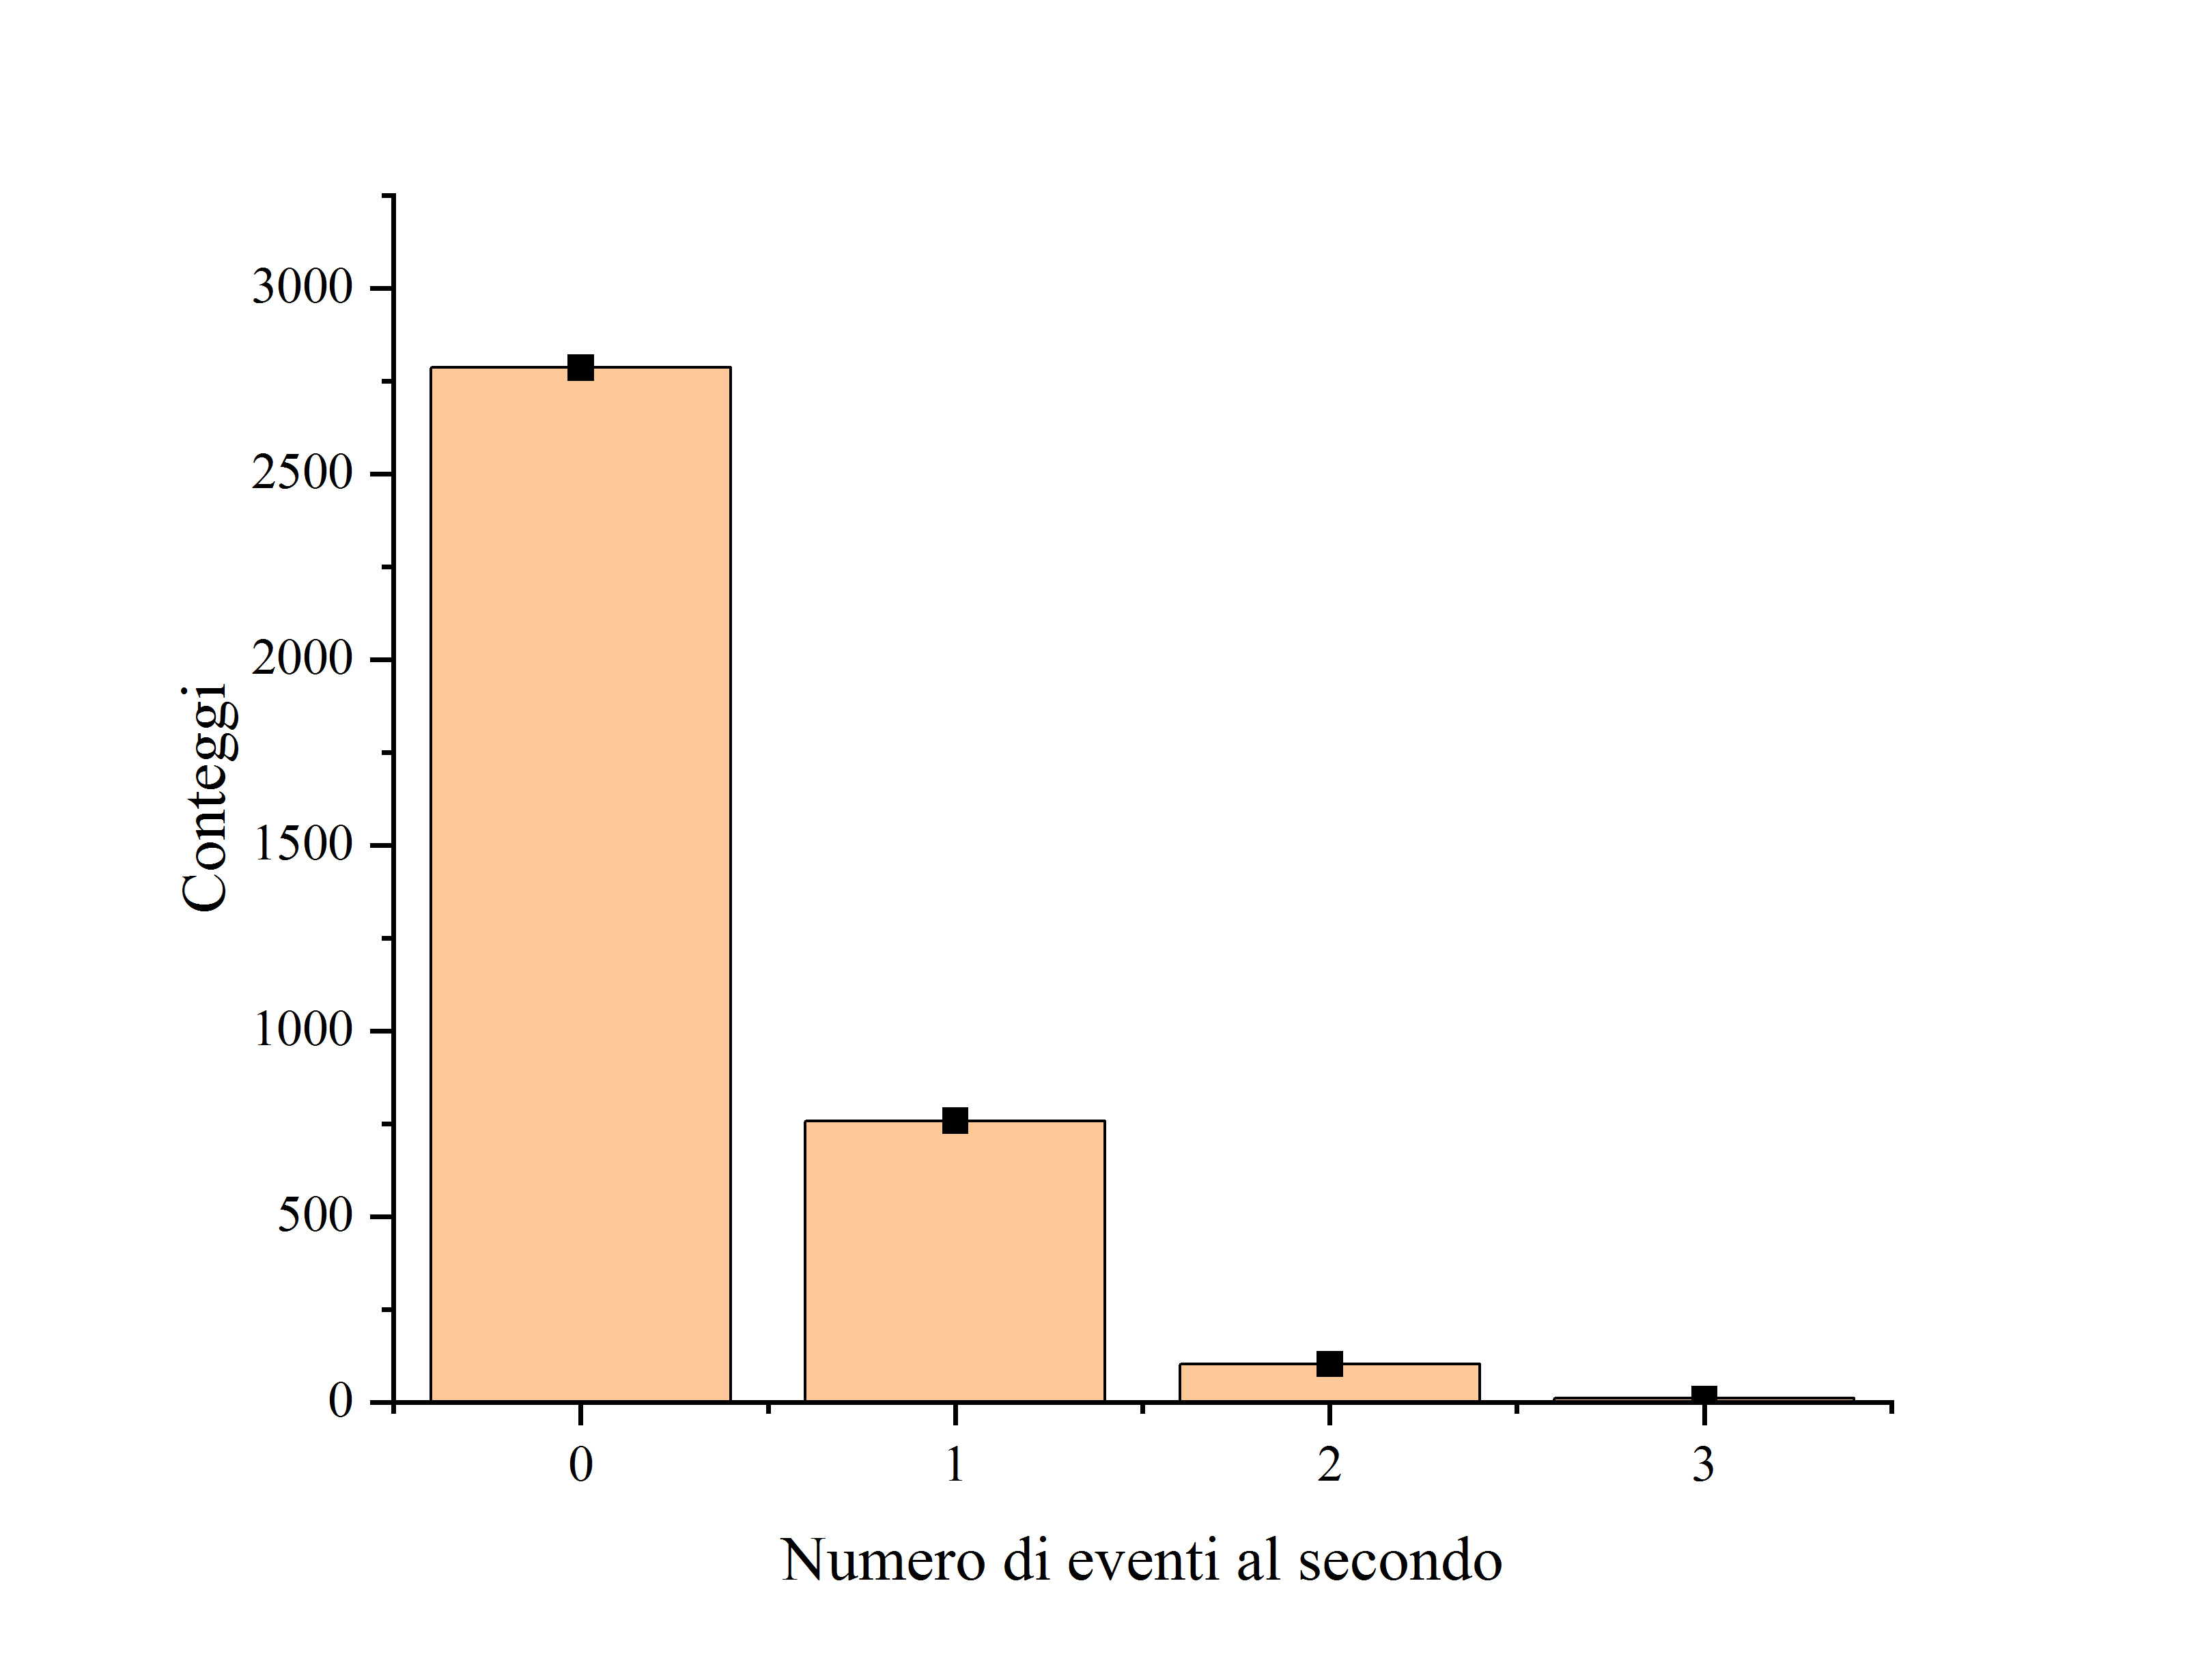
\includegraphics[trim={2cm .5cm 2.4cm 2.1cm},clip,width=.5\textwidth]{img/Geiger4.jpg}
        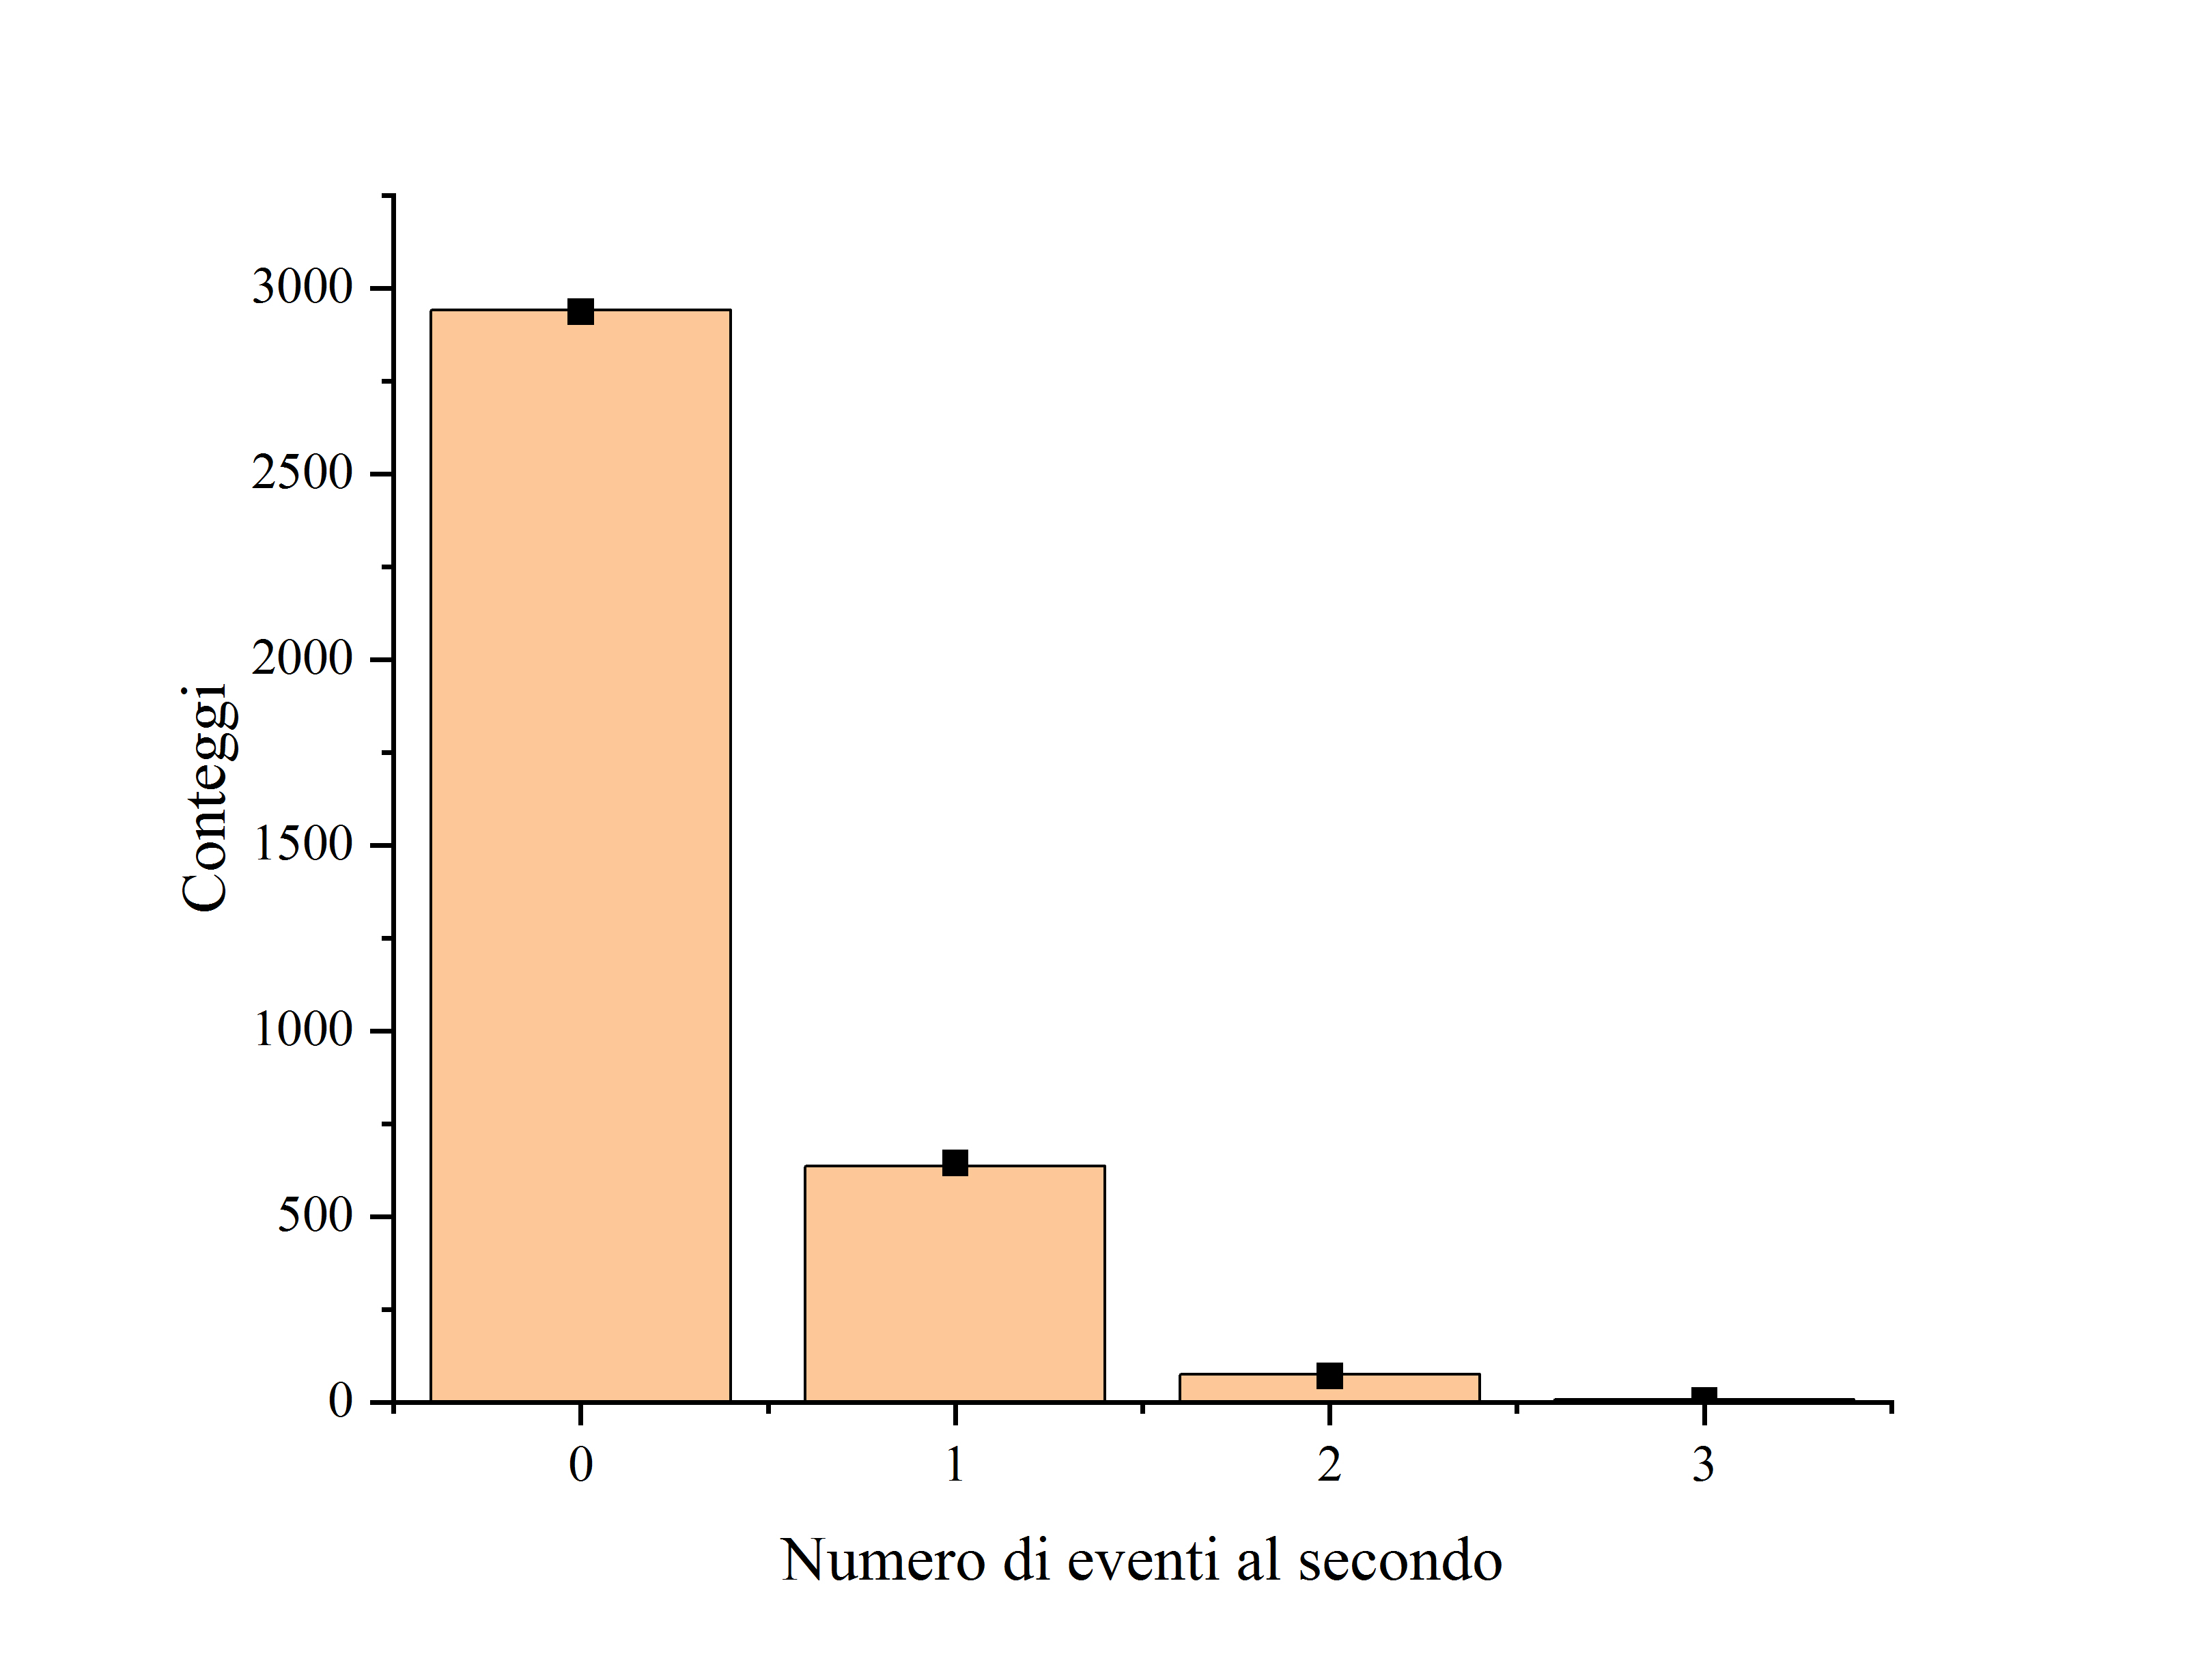
\includegraphics[trim={2cm .5cm 2.4cm 2.1cm},clip,width=.5\textwidth]{img/Geiger5.jpg}
    \end{figure}\begin{figure}[H]
        \centering
        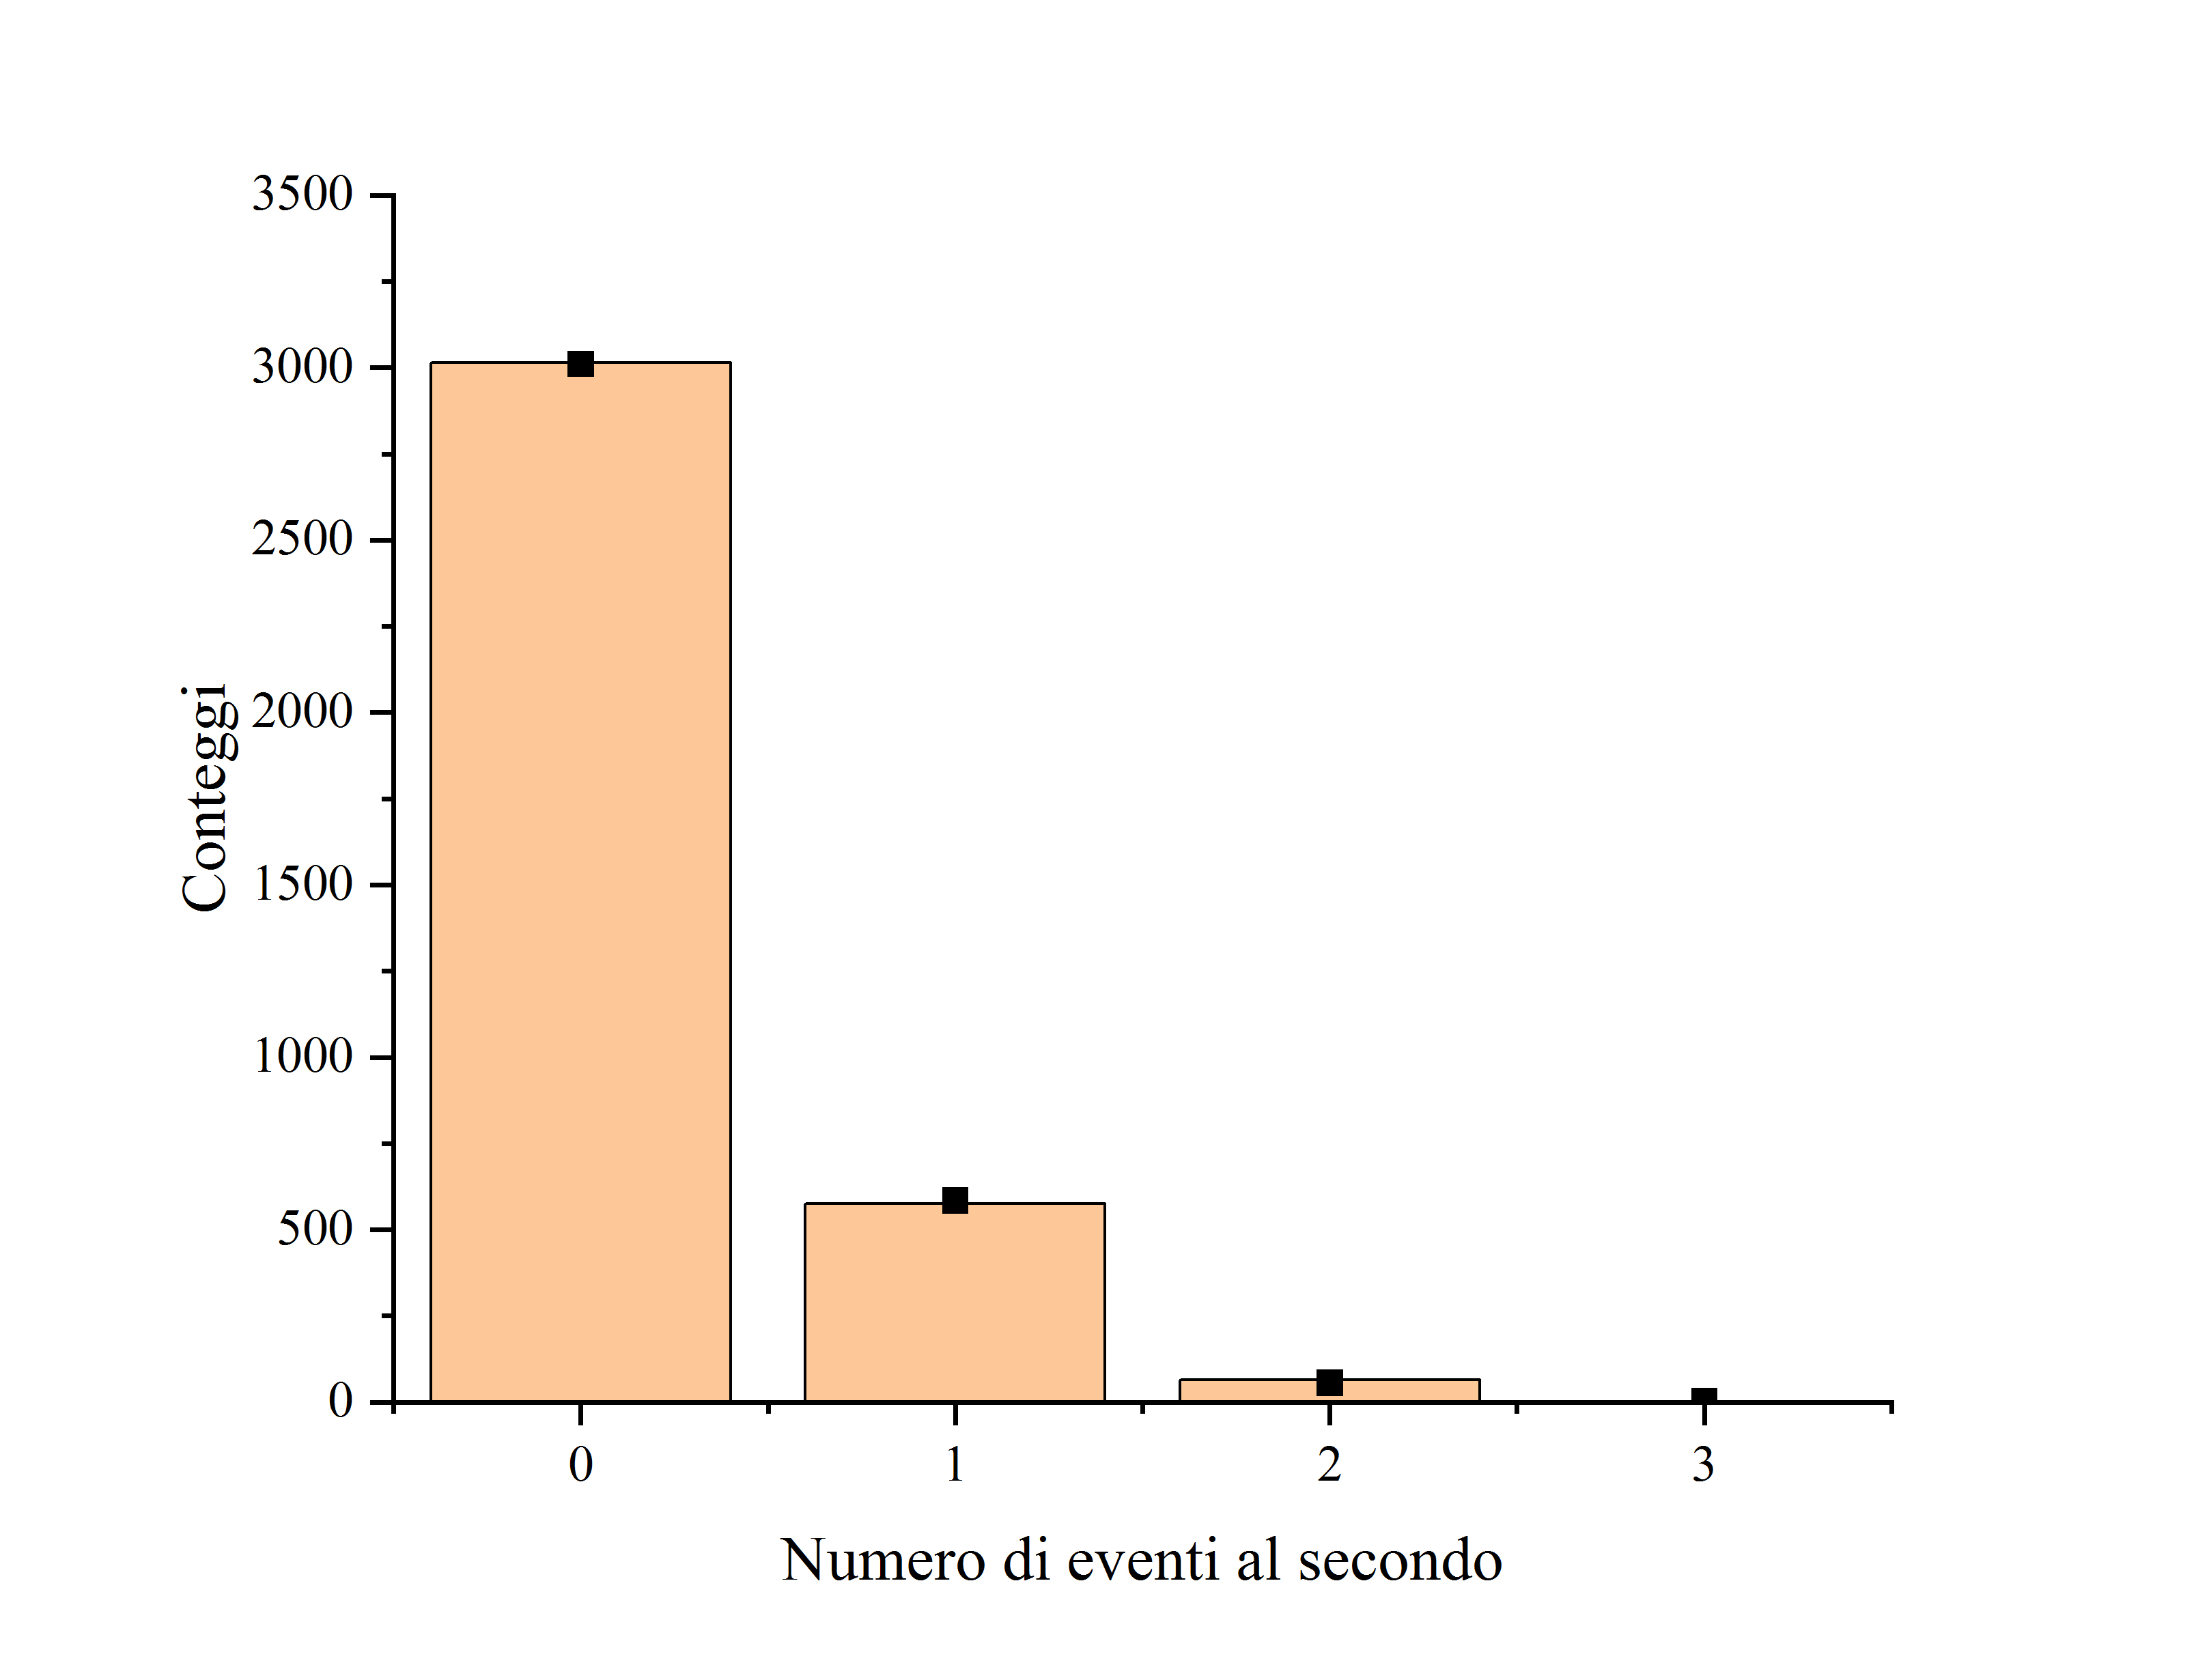
\includegraphics[trim={2cm .5cm 2.4cm 2.1cm},clip,width=.5\textwidth]{img/Geiger0.jpg}
        \caption*{Conteggi, nell'ordine, di $x_1$, $x_2$, $x_3$, $x_4$ e $x_0$.}
    \end{figure}
\end{center}

Come si può osservare da questi grafici, i risultati ottenuti si allineano molto bene
alle distribuzioni di Poisson.

In particolare, $\overline{x_0} = \left(194\pm7\right)\cdot10^{-3}\,\unit{s^{-1}}$.

Per valutare l'accuratezza della nostra stima di $\overline{x_0}$, possiamo effettuare
una regressione lineare (pesata) utilizzando l'equazione di $x_i$ in funzione di
$d_i^{-2}$: \[\overline{x_i} = \xi d_i^{-2} + \overline{x_0}\]
Di seguito riportiamo una tabella con i dati utilizzati per la regressione lineare\footnote{
    Tutti gli errori, qui e successivamente, sono stati calcolati secondo la tradizionale
    propagazione degli errori, in quanto sono considerabili piccoli, casuali e indipendenti.
}, assieme a un grafico della retta di regressione stessa.

\begin{center}
    \begin{tblr}{ |Q[c,m]|Q[c,m]|Q[c,m]|Q[c,m]| }
        \hline
        $i$ & $d_i\;\;(\unit{cm})$ & $d_i^{-2}\;\;(\unit{m^{-2}})$ & $\overline{x_i}\;\;(\unit{s^{-1}})$ \\
        \hline
        1 & $9.5\pm0.1$  & $111\pm2$      & $0.809\pm0.015$\\
        2 & $10.3\pm0.1$ & $94.3\pm1.8$   & $0.737\pm0.014$\\
        3 & $26.5\pm0.1$ & $14.24\pm0.11$ & $0.272\pm0.009$\\
        4 & $41.2\pm0.1$ & $5.89\pm0.03$  & $0.219\pm0.008$\\
        \hline
    \end{tblr}
    \begin{figure}[H]
        % trim={< v > ^}
        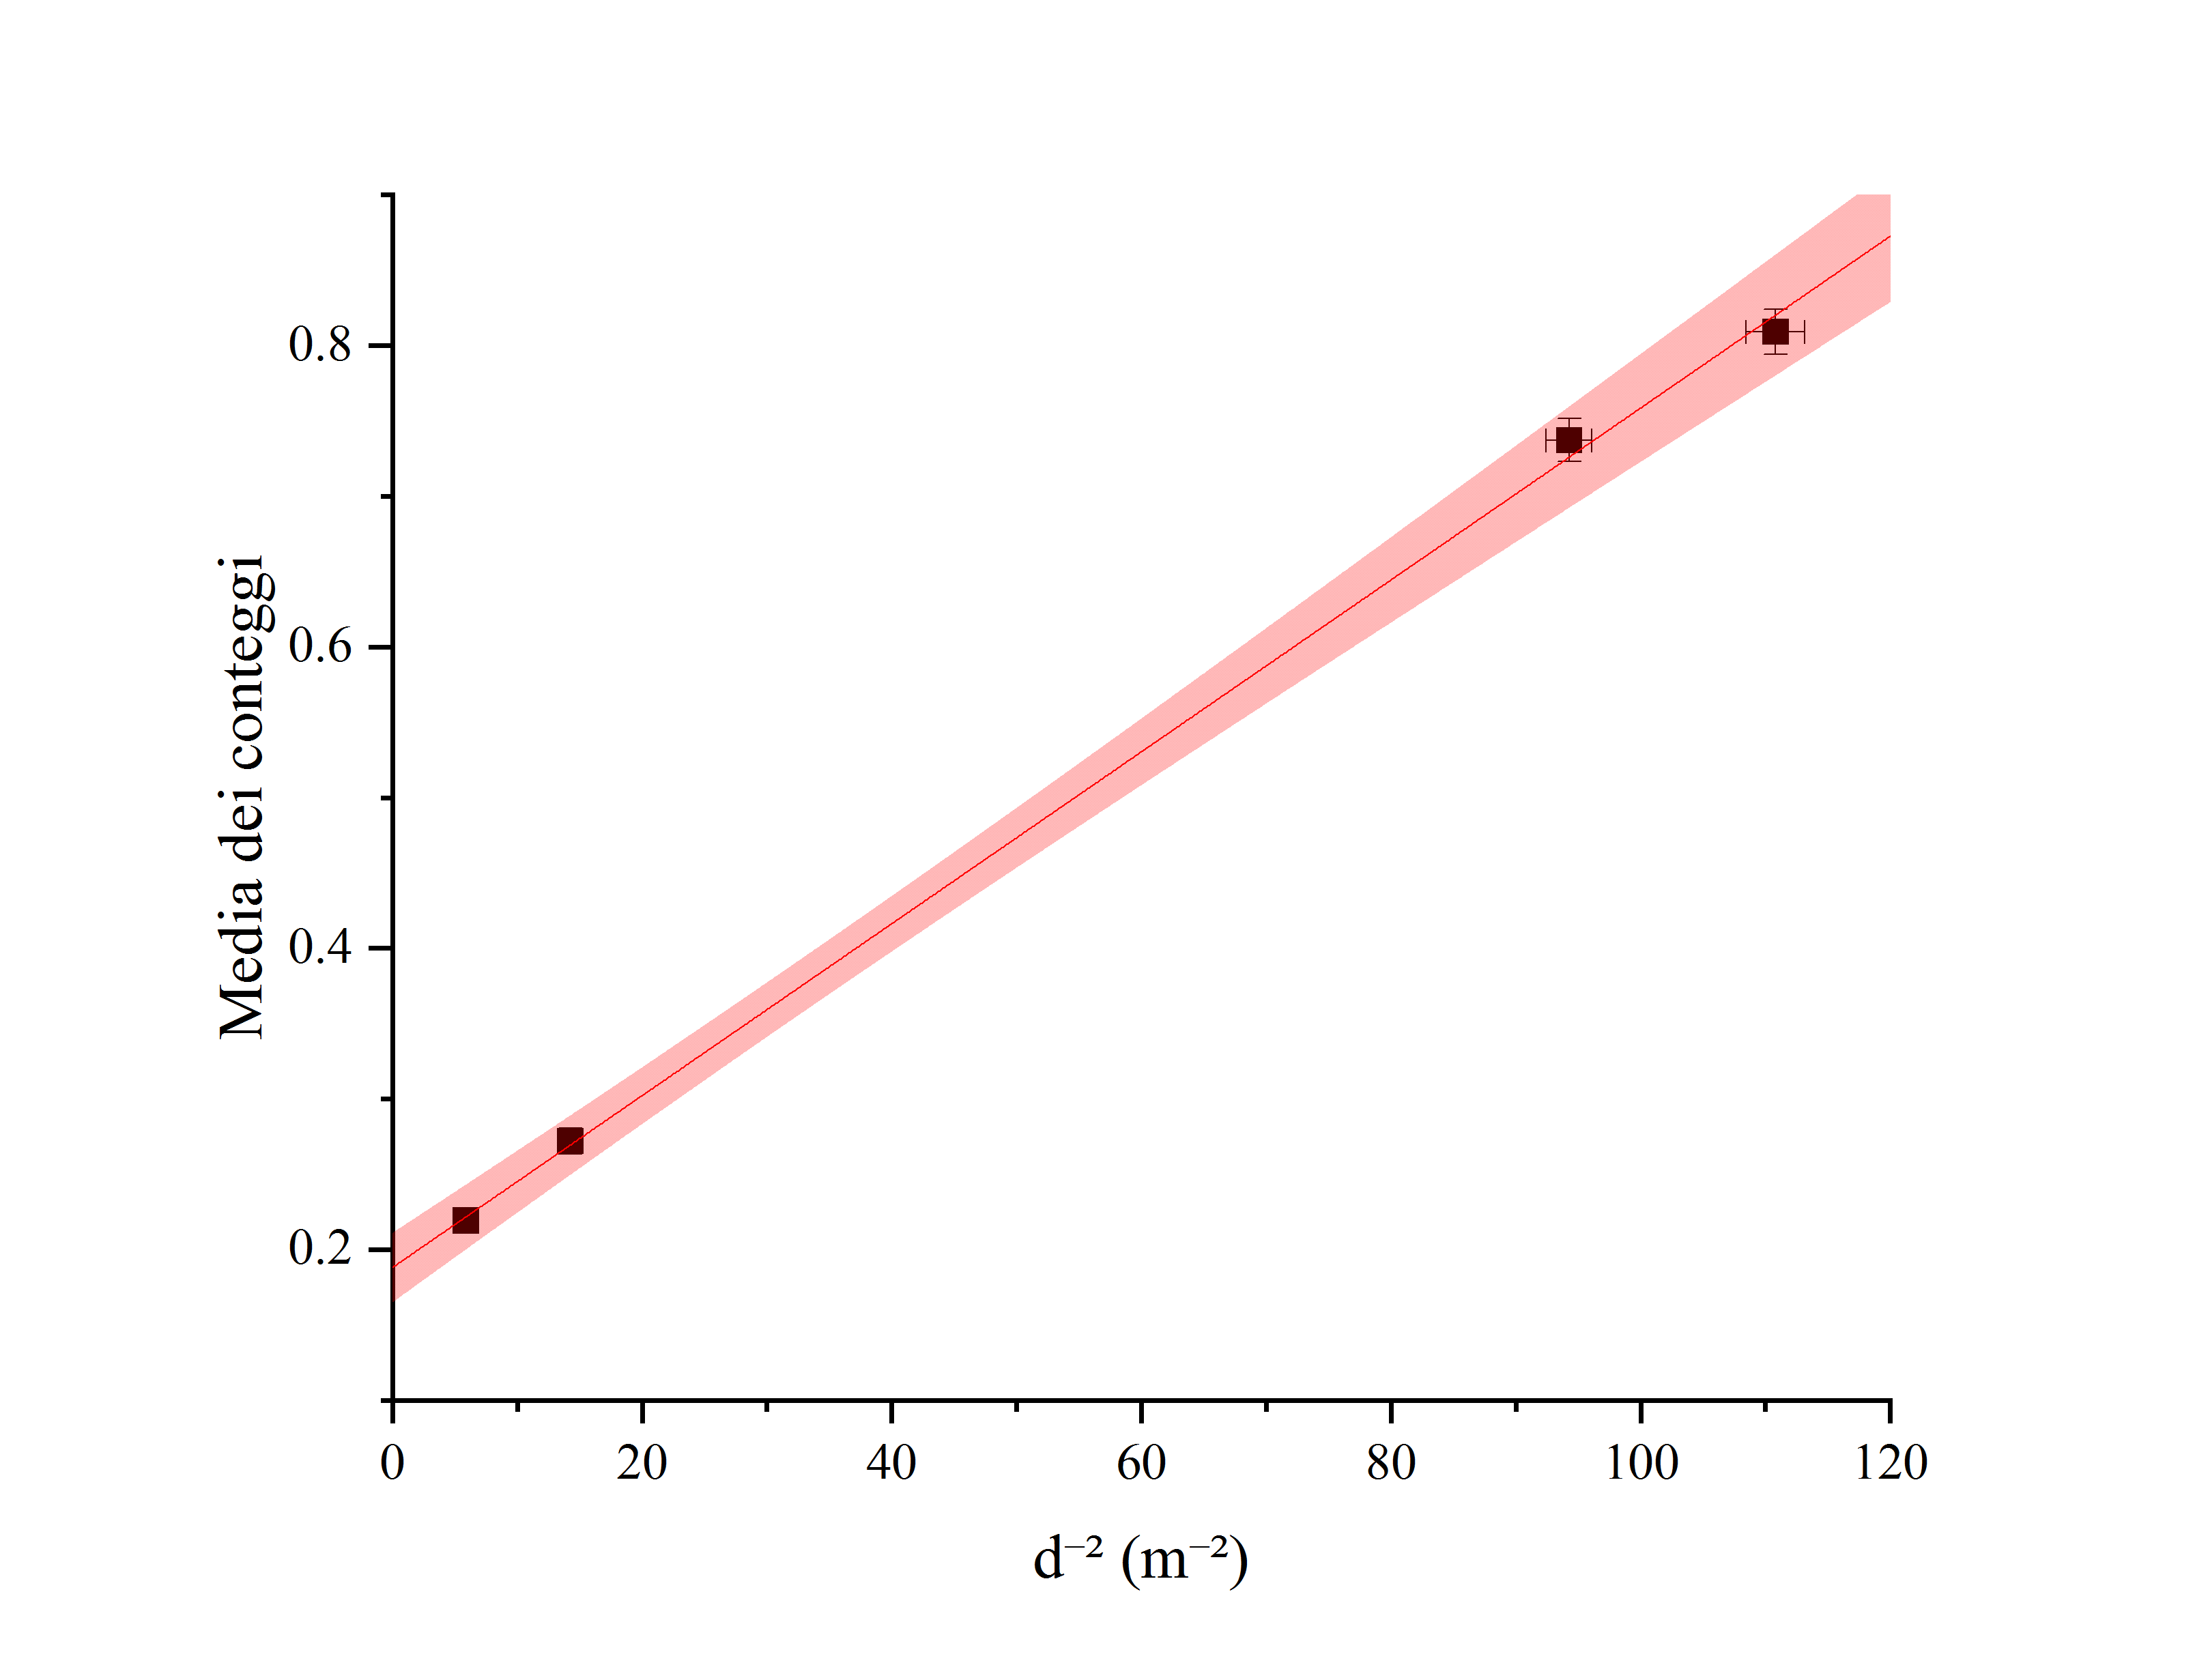
\includegraphics[trim={2cm .5cm 2cm 2.1cm},clip,width=\textwidth]{img/Regressione.png}
        \caption*{Regressione lineare. In rosa la regione di incertezza.}
    \end{figure}
\end{center}

Risultati della regressione lineare:
\begin{itemize}
    \item $\overline{x_0} = \left(188\pm6\right)\cdot10^{-3}\,\unit{s^{-1}}$ (intercetta)
    \item $\xi = \left(5.70\pm0.13\right)\cdot10^{-3}\,\unit{m^2\per s}$ (coefficiente angolare)
\end{itemize}

Per valutare numericamente la consistenza tra i due valori di $\overline{x_0}$
ottenuti ($\overline{x_0}_\text{\,diretto}$, misurato direttamente, e
$\overline{x_0}_\text{\,indiretto}$, ottenuto dalla regressione lineare),
abbiamo calcolato il seguente valore (numero puro):
\[
    \varepsilon =
    \frac{
        \left(\overline{x_0}_\text{\,diretto}\right)_\text{best} -
        \left(\overline{x_0}_\text{\,indiretto}\right)_\text{best}
    }{
        \delta\overline{x_0}_\text{\,diretto} +
        \delta\overline{x_0}_\text{\,indiretto}
    }
\]
Allora $\overline{x_0}_\text{\,diretto}$ e $\overline{x_0}_\text{\,indiretto}$
sono consistenti se e solo se $\left|\varepsilon\right|\le1$.

Nel nostro caso, $\varepsilon = +0.45$, per cui i due valori di $\overline{x_0}$
sono consistenti.

Dal valore di $\xi$ ottenuto mediante la regressione lineare, è possibile stimare
il numero $N$ di atomi (e, di conseguenza, la massa) di $\Th$ nel campione.

Dalle formule precedentemente esposte, segue:
\[
    N = \frac{4\,\xi\,T_\frac{1}{2}}{r^2\ln{2}}
    = \left(2.98\pm0.09\right)\cdot10^{20}
\]
da cui:
\[\begin{aligned}
    m &= m_{\left(\text{1 atomo di }\Th\right)}N
       = (90(m_p+m_e) + (232-90)m_n)N\\
      &= \left(1.16\pm0.04\right)\cdot10^{-4}\,\unit{kg}
       = \left(0.116\pm0.004\right)\unit{g}
       = \left(116\pm4\right)\unit{mg}.
\end{aligned}\]

\pagebreak
\begin{appendices}

\section{Onestà dei dadi}
Per prima cosa, mostreremo e giustificheremo il procedimento che abbiamo utilizzato per
determinare se ogni dado sia onesto; successivamente, riporteremo i risultati di questa
analisi statistica operata sui singoli dadi.

\subsection{Analisi statistica: motivazione}

\subsubsection{Sommario}
Sia $D$ un dado a $N\in\left[2,+\infty\right)\cap\mathbb{N}$ facce distinte
$D_1,\dots,D_N$ con probabilità di uscire in un solo lancio, rispettivamente,
$p_1,\dots,p_N\in\left[0;1\right]$.

Consideriamo $n\in\mathbb{N}$ lanci ripetuti di $D$.
Per ogni faccia $D_i$, chiameremo $n_i$ il numero di occorrenze di $D_i$.

Per valutare se $D$ è truccato, ci limiteremo a studiare separatamente le $N$ facce:
riterremo il dado “truccato” se e solo se almeno una delle facce è “truccata”.
Diremo una faccia $D_i$ “truccata” se e solo se la probabilità che $p_i$ sia “pari a $\frac{1}{N}$
o peggio”, in base ai dati raccolti, è inferiore al $5\%$.

Chiariremo in seguito questi termini, ove opportuno.

\subsubsection{Notazione generale}
In questa sede, indicheremo con $p(A)$ la probabilità dell'evento $A$ e con $p(A|E)$ la
probabilità di $A$ condizionata al verificarsi dell'evento $E$.

Nel caso di distribuzioni continue, indicheremo con $f_X$ la funzione di densità di probabilità
della variabile aleatoria $X$.
Pertanto, fissato $\left[x_1;x_2\right]\subseteq\left[0;1\right]$, vale:
\[p(x_1\le X\le x_2) = \int_{x_1}^{x_2}f_X(x)\,dx.\]

Analogamente, $f_{X|E}$ sarà la funzione di densità di probabilità della variabile aleatoria $X$
condizionata al verificarsi dell'evento $E$ e varrà, come prima:
\[p(x_1\le X\le x_2|E) = \int_{x_1}^{x_2}f_{X|E}(x)\,dx.\]

\subsubsection{Lanci consecutivi: distribuzione di Bernoulli}

Limitiamoci a studiare le occorrenze di ogni faccia $D_i$ separatamente.

Trattando gli $n$ lanci come prove di Bernoulli con probabilità di successo $p_i$, al variare di
$x\in\left[0;1\right]$ la probabilità che $D_i$ si presenti
$m\in\left\{1,\dots,n\right\}$ volte fra gli $n$ lanci sarà allora:
\[p(n_i=m|p_i=x) = \binom{n}{m} x^m (1-x)^{n - m}.\]

Tuttavia, per stimare l'onestà della faccia $D_i$, è necessario determinare la distribuzione di
probabilità di $p_i$ in base ai dati raccolti, cioè passare dalla funzione
$x\longmapsto p(n_i=m|p_i=x)$ alla funzione $x\longmapsto f_{p_i|n_i=m}(x)$.

\subsubsection{Il teorema di Bayes}
È possibile operare questo cambio di prospettiva mediante il teorema di Bayes sulla probabilità
condizionata, ricordando che, nel caso di distribuzioni continue, esso opera sulle funzioni di
densità di probabilità:

\[f_{p_i|n_i=m}(x) = \frac{p(n_i=m|p_i=x)\;f_{p_i}(x)}{p(n_i=m)}.\]

\emph{
    \textbf{Nota.} Non stiamo più lavorando con distribuzioni discrete, bensì continue,
    poiché $p_i \in \left[0,1\right]$ è la nostra (nuova) variabile aleatoria.
    Questo è corretto, in quanto, ad esempio, non avrebbe senso lavorare su
    $p(p_i = \frac{1}{6}|n_i=m)$, poiché sarebbe sempre $0$: in fondo, è impossibile
    costruire un dado “perfettamente onesto” senza margini di errore!
}

Supponiamo che la distribuzione \emph{a priori} di $p_i$ sia uniforme, per cui:
\[f_{p_i}(x) = 1\qquad\forall x\in \left[0,1\right].\]
e quindi:
\[p(x_1\le p_i\le x_2) = \int_{x_1}^{x_2}1\,dx = x\Big|_{x_1}^{x_2}=x_2-x_1
\qquad\forall \left[x_1,x_2\right]\subseteq \left[0,1\right].\]
Calcoliamo allora\footnote{
In generale, $\int_{0}^{1}x^a(1-x)^b\,dx = \frac{a!\,b!}{(a+b+1)!}\quad\forall a,b\in\mathbb{N}$.
Ciò si dimostra, ad esempio, per induzione su $b$, utilizzando, nel passo induttivo, l'integrazione
per parti.

Tuttavia, questa famiglia di integrali non ammette un'espressione analitica “chiusa”
nel caso indefinito: questo è il motivo per cui \emph{non} tenteremo di determinare l'espressione
generale di $p(x_1\le p_i\le x_2|n_i=m)$, facendo affidamento, invece, a metodi numerici.
} $p(n_i=m)$:
\[\begin{aligned}
p(n_i=m)&=p(n_i=m|0\le p_i\le 1) = \int_{0}^{1}p(n_i=m|p_i=x)\,dx=\\
        &=\int_{0}^{1}\binom{n}{m}x^m (1-x)^{n - m}\,dx=\binom{n}{m}\int_{0}^{1}x^m(1-x)^{n - m}\,dx=\\
        &=\binom{n}{m}\frac{m!\;(n-m)!}{(n+1)!}
        =\frac{n!}{m!\;(n-m)!}\cdot\frac{m!\;(n-m)!}{(n+1)\,n!}
        =\frac{1}{n+1}
\end{aligned}\]
Sostituendo quanto appena trovato nell'espressione di $f_{p_i|n_i=m}$, otteniamo:
\[f_{p_i|n_i=m}(x)=\frac{\binom{n}{m}x^m(1-x)^{n-m}\cdot 1}{\frac{1}{n+1}}
=\frac{(n+1)!}{m!\;(n-m)!}\,x^m(1-x)^{n-m}.\]

\subsubsection{La nuova distribuzione}
Si può osservare che quella trovata è, come ci si aspetterebbe, una distribuzione di probabilità:
\[\begin{aligned}
p(0\le p_i\le 1|n_i=m)  &= \int_{0}^{1}f_{p_i|n_i=m}(x)\,dx = \\
                        &= \frac{(n+1)!}{m!\;(n-m)!}\int_{0}^{1}x^m(1-x)^{n-m}\,dx = \\
                        &= \frac{(n+1)!}{m!\;(n-m)!}\cdot\frac{m!\;(n-m)!}{(n+1)!} = 1
\end{aligned}\]
La media di questa distribuzione è:
\[\begin{aligned}
\mu \coloneqq \mu_{p_i|n_i=m} &= \int_{0}^{1}xf_{p_i|n_i=m}(x)\,dx = \\
    &= \frac{(n+1)!}{m!\;(n-m)!}\int_{0}^{1}x^{m+1}(1-x)^{n-m}\,dx = \\
    &= \frac{(n+1)!}{m!\;(n-m)!}\cdot\frac{(m+1)!\;(n-m)!}{(n+2)!} =
    \frac{m+1}{n+2}
\end{aligned}\]
La sua varianza, invece, è\footnote{
Per brevità, non riportiamo tutti i passaggi della risoluzione. L'integrale è stato
calcolato espandendo il quadrato del binomio e poi procedendo con i tre integrali definiti
risultanti come accennato alla nota 8.
}:
\[\begin{aligned}
\sigma_{p_i|n_i=m}^2 &= \int_{0}^{1}(x-\mu_{p_i|n_i=m})^2f_{p_i|n_i=m}(x)\,dx = \\
&= \frac{(n+1)!}{m!\;(n-m)!}\int_{0}^{1}\left(x-\frac{m+1}{n+2}\right)^2x^{m+1}(1-x)^{n-m}\,dx = \\
&= \frac{m+1}{n+2}\left(\frac{m+2}{n+3}-\frac{m+1}{n+2}\right)
\end{aligned}\]

\subsubsection{La faccia $D_i$ è onesta?}
Per valutare l'onestà della faccia $D_i$, abbiamo ritenuto opportuno basarci sulla probabilità
che $p_i$ sia “$\frac{1}{N}$ o peggio”. Più formalmente, detto:
\[\Delta x \coloneqq \left|\frac{1}{N} - \mu\right|\]
chiameremo “onestà di $D_i$” il valore:
\[\begin{aligned}
\omega_{D_i|n_i=m} &\coloneqq p(p_i\in\left[0;\mu-\Delta x\right)\cup\left(\mu+\Delta x;1\right])=\\
    &=1-p(p_i\in\left[\mu-\Delta x;\mu+\Delta x\right])=\\
    &=1-\int_{\mu-\Delta x}^{\mu+\Delta x}f_{p_i|n_i=m}(x)\,dx.
\end{aligned}\]
In particolare, diremo che la faccia è “truccata” se $\omega_{D_i|n_i=m}<5\%$.

Tuttavia, con $n$ finito, non possiamo valutare \emph{con certezza} l'onestà della faccia.
Per avere una stima della \emph{precisione} della nostra valutazione, calcoliamo anche\footnote{
    Per $m=0$ o $m=n$, una delle due espressioni non ha senso. Per ovviare a ciò,
    basta definire $\omega_{D_i|n_i=n+1}\coloneqq0$ e $\omega_{D_i|n_i=-1}\coloneqq0$.
}
$\omega_{D_i|n_i=m-1}$ e $\omega_{D_i|n_i=m+1}$; allora:
\begin{itemize}
    \item Se tutte e tre le probabilità sono $<5\%$, diremo che
          “\emph{è abbastanza probabile che $D_i$ sia truccata}”.
    \item Se tutte e tre le probabilità sono $\ge5\%$, diremo che
          “\emph{non è abbastanza probabile che $D_i$ sia truccata}”.
    \item Altrimenti, diremo che
          “\emph{$D_i$ potrebbe essere truccata, ma $n$ lanci sono troppo pochi per poterlo
          affermare ragionevolmente}”.
\end{itemize}
Questa interpretazione di $\omega_{D_i|n_i=m}$, $\omega_{D_i|n_i=m-1}$ e $\omega_{D_i|n_i=m+1}$
è giustificata dalle seguenti proposizioni (dimostrabili):
\[\omega_{D_i|n_i=m-1}\le\omega_{D_i|n_i=m}\le\omega_{D_i|n_i=m+1}\]
\[\vee\]
\[\omega_{D_i|n_i=m-1}\ge\omega_{D_i|n_i=m}\ge\omega_{D_i|n_i=m+1}\]

\[
    \lim_{n\rightarrow+\infty}\omega_{D_i|n_i=m-1} =
    \lim_{n\rightarrow+\infty}\omega_{D_i|n_i=m} =
    \lim_{n\rightarrow+\infty}\omega_{D_i|n_i=m+1}
\]

Infine, diremo che “$D$ è truccato” se e solo se almeno una faccia è truccata. Più formalmente:
\begin{itemize}
    \item Se $\exists D_i$ tale che è abbastanza probabile che $D_i$ sia truccata,
          diremo che “\emph{è abbastanza probabile che $D$ sia truccato}”.
    \item Se $\forall D_i$ non è abbastanza probabile che $D_i$ sia truccata,
          diremo che “\emph{non è abbastanza probabile che $D$ sia truccato}”.
    \item Altrimenti, diremo che
          “\emph{$D$ potrebbe essere truccato, ma $n$ lanci sono troppo pochi per poterlo
          affermare ragionevolmente}”.
\end{itemize}

\emph{\textbf{Osservazione.} Le variabili aleatorie $p_1,\dots,p_N$ non sono fra loro indipendenti:
infatti, per ovvi motivi, deve valere $p_1+\dots+p_N = 1$. Pertanto, in generale:}
\[p(D\text{ onesto})=p\left(\bigcap_{i=1}^N D_i\text{ onesta}\right)
\ne\prod_{i=1}^{N}p(D_i\text{ onesta})\]
\emph{Si potrebbe definire una funzione a $N$ variabili
$F:\left[0,1\right]^N\longrightarrow\left[0,1\right]$, ad esempio:}
\[F(x_1,\dots,x_n) = \sqrt{N}\left\lVert
\begin{bmatrix}x_1\\\vdots\\x_N\end{bmatrix} - \frac{1}{N}\begin{bmatrix}1\\\vdots\\1\end{bmatrix}
\right\rVert = \sqrt{N\sum_{i=1}^{N}\left(x_i-\frac{1}{N}\right)^2}\]
\emph{per poi determinare i valori che $p_1,\dots,p_n$ devono assumere affinché, ad esempio,
$F(p_1,\dots,p_n)\le95\%$. Il problema, allora, sarebbe calcolare le probabilità che
$p_1,\dots,p_n$ assumano tali valori, in quanto, come detto, non sono fra loro indipendenti.}

\emph{Alla luce di queste osservazioni, il gruppo di lavoro ha ritenuto pertanto
opportuno valutare l'onestà del dado considerando le singole facce separatamente.
Si tratta, in un certo senso, di una sovrastima: se almeno una faccia è “truccata”
(indipendentemente dalle altre), anche tutto il dado è “truccato”; se il dado è
“truccato”, non è detto che la nostra stima lo valuti come tale, perché ogni faccia
potrebbe comunque risultare “onesta”, quando considerata indipendentemente dalle
altre.}

\emph{Bisogna infine osservare che la definizione di “onestà” è piuttosto
arbitraria, o, comunque, non univoca: questo giustifica ulteriormente la
nostra conduzione dell'analisi dell'“onestà” dei dadi.}

\subsection{I nostri dadi sono truccati?}
Riportiamo finalmente i parametri della nostra analisi valutati sui dati raccolti
($N = 400$).
Gli integrali sono stati valutati con metodi numerici, in particolare mediante
somme di Riemann su intervalli sufficientemente piccoli.

\begin{center}
    \begin{tblr}{ |Q[c,m]|Q[c,m]|Q[c,m]|Q[c,m]|Q[c,m]|Q[c,m]| }
        \hline
        $i$ & $m$ & $\omega_{D_i|n_i=m-1}$ & $\omega_{D_i|n_i=m}$ & $\omega_{D_i|n_i=m+1}$ & Conclusione \\
        \hline
        \hline
        \SetCell[c=5]{c} { Dado rosso } & {Truccato} \\
        \hline
        1 &  & 1.044\% & 1.644\% & 2.535\% & Truccata \\
        2 &  & 8.077\% & 6.252\% & 4.795\% & N./A. \\
        3 &  & 89.429\% & 79.157\% & 69.339\% & Onesta \\
        4 &  & 3.817\% & 5.602\% & 8.006\% & N./A. \\
        5 &  & 2.053\% & 1.522\% & 1.120\% & Truccata \\
        6 &  & 48.983\% & 58.329\% & 68.280\% & Onesta \\
        \hline
        \hline
    \end{tblr}
\end{center}

\pagebreak
\section{Codice Rust per $10^{12}$ lanci di sei dadi}

Qui riportiamo il codice Rust, da noi scritto, che ci ha permesso di
lanciare virtualmente $6\cdot10^{12}$ dadi in maniera estremamente
efficiente.

\inputminted[linenos, mathescape]{rust}{src/main.rs}

\end{appendices}
\end{document}
